% !TEX program = XeLaTeX (custom)
\documentclass[14pt,a4paper,oneside]{extbook}

%% --- Thai --- %
% Set up fonts and encoding
\usepackage{fontspec}
\usepackage{xunicode}
\usepackage{xltxtra}

% Enable line breaks for Thai text
\XeTeXlinebreaklocale "th"
\XeTeXlinebreakskip = 0pt plus 2pt minus 1pt

% Set up Thai fonts
\setmainfont[%
    ItalicFont={Thasadith Italic},%
    BoldFont={Thasadith Bold},%
    BoldItalicFont={Thasadith Italic},%
    Script=Thai,%
    Scale=MatchLowercase,%
    WordSpace=1.25,%
    Mapping=tex-text,%
]{Thasadith}

%% --- %%

\usepackage{etoolbox}
\usepackage[a4paper,top=1.25in,bottom=1.25in,left=1in,right=1in]{geometry}
\usepackage{indentfirst}
\usepackage{apacite}
\usepackage{enumitem}
\usepackage{titlesec}
\usepackage{tabu}
\usepackage[most]{tcolorbox}
\tcbuselibrary{minted}
\usepackage{float}
\usepackage{graphicx}
\usepackage{caption}
\usepackage{fancyhdr}
\usepackage{hanging}
\usepackage{appendix}

\definecolor{darkblue}{RGB}{14,77,146}


% \titleformat{\chapter}
% {\color{darkblue}\normalfont\Huge\bfseries}
% {\color{darkblue}\thechapter}{1em}{}

% \titleformat{\section}
% {\color{darkblue}\normalfont\Large\bfseries}
% {\color{darkblue}\thesection}{1em}{}

\captionsetup[table]{skip=10pt}
\graphicspath{{./images/}}
\setlist[itemize]{noitemsep,nolistsep,topsep=0pt}

\pagestyle{fancy}
\fancyhf{}
\fancyhead[LE,RO]{เวอร์ชัน 1.63.1.2 \hfill\nouppercase\leftmark}
\fancyfoot[LE,RO]{ดร.จันทวรรณ ปิยะวัฒน์\hfill \thepage}
\renewcommand{\headrulewidth}{2pt}
% \renewcommand{\headrule}{\hbox to\headwidth{\color{darkblue}\leaders\hrule height \headrulewidth\hfill}}
\renewcommand{\footrulewidth}{1pt}
% \renewcommand{\footrule}{\hbox to\headwidth{\color{darkblue}\leaders\hrule height \footrulewidth\hfill}}

\makeatletter
\patchcmd{\f@nch@head}{\rlap}{\color{darkblue}\rlap}{}{}
\patchcmd{\headrule}{\hrule}{\color{darkblue}\hrule}{}{}
\patchcmd{\f@nch@foot}{\rlap}{\color{darkblue}\rlap}{}{}
\patchcmd{\footrule}{\hrule}{\color{darkblue}\hrule}{}{}
\makeatother

\titleformat{\chapter}[display]
%\titleclass{\chapter}{straight}
{\normalfont\huge\bfseries}{\chaptertitlename\ \thechapter}{0pt}{\Huge}
\titlespacing*{\chapter}{0pt}{-50pt}{0pt}
\titlespacing{\chapter}{0pt}{-50pt}{0pt}


\usepackage{minted}
\setminted{fontsize=\small,baselinestretch=1,startinline=true}
\newminted{py}{python3,linenos=true,escapeinside=||}

\renewcommand{\baselinestretch}{1.5}
\renewcommand{\contentsname}{สารบัญ}
\renewcommand{\chaptername}{บทที่}
\renewcommand{\listfigurename}{สารบัญรูป}
\renewcommand{\figurename}{รูปที่}
\renewcommand{\listtablename}{สารบัญตาราง}
\renewcommand{\tablename}{ตารางที่}

%https://tex.stackexchange.com/a/343366
\newenvironment{codelist}[3][]
 {\VerbatimEnvironment
  % \begin{figure}[H]
  % \caption{#2}\label{#3}
  \begin{minted}[xleftmargin=\parindent,linenos,escapeinside=||]{python3}}
 {
   \end{minted}
  % \end{figure}
  }

\begin{document}

\newmintinline{py}{python3}

\frontmatter
\begin{titlepage}
\centering
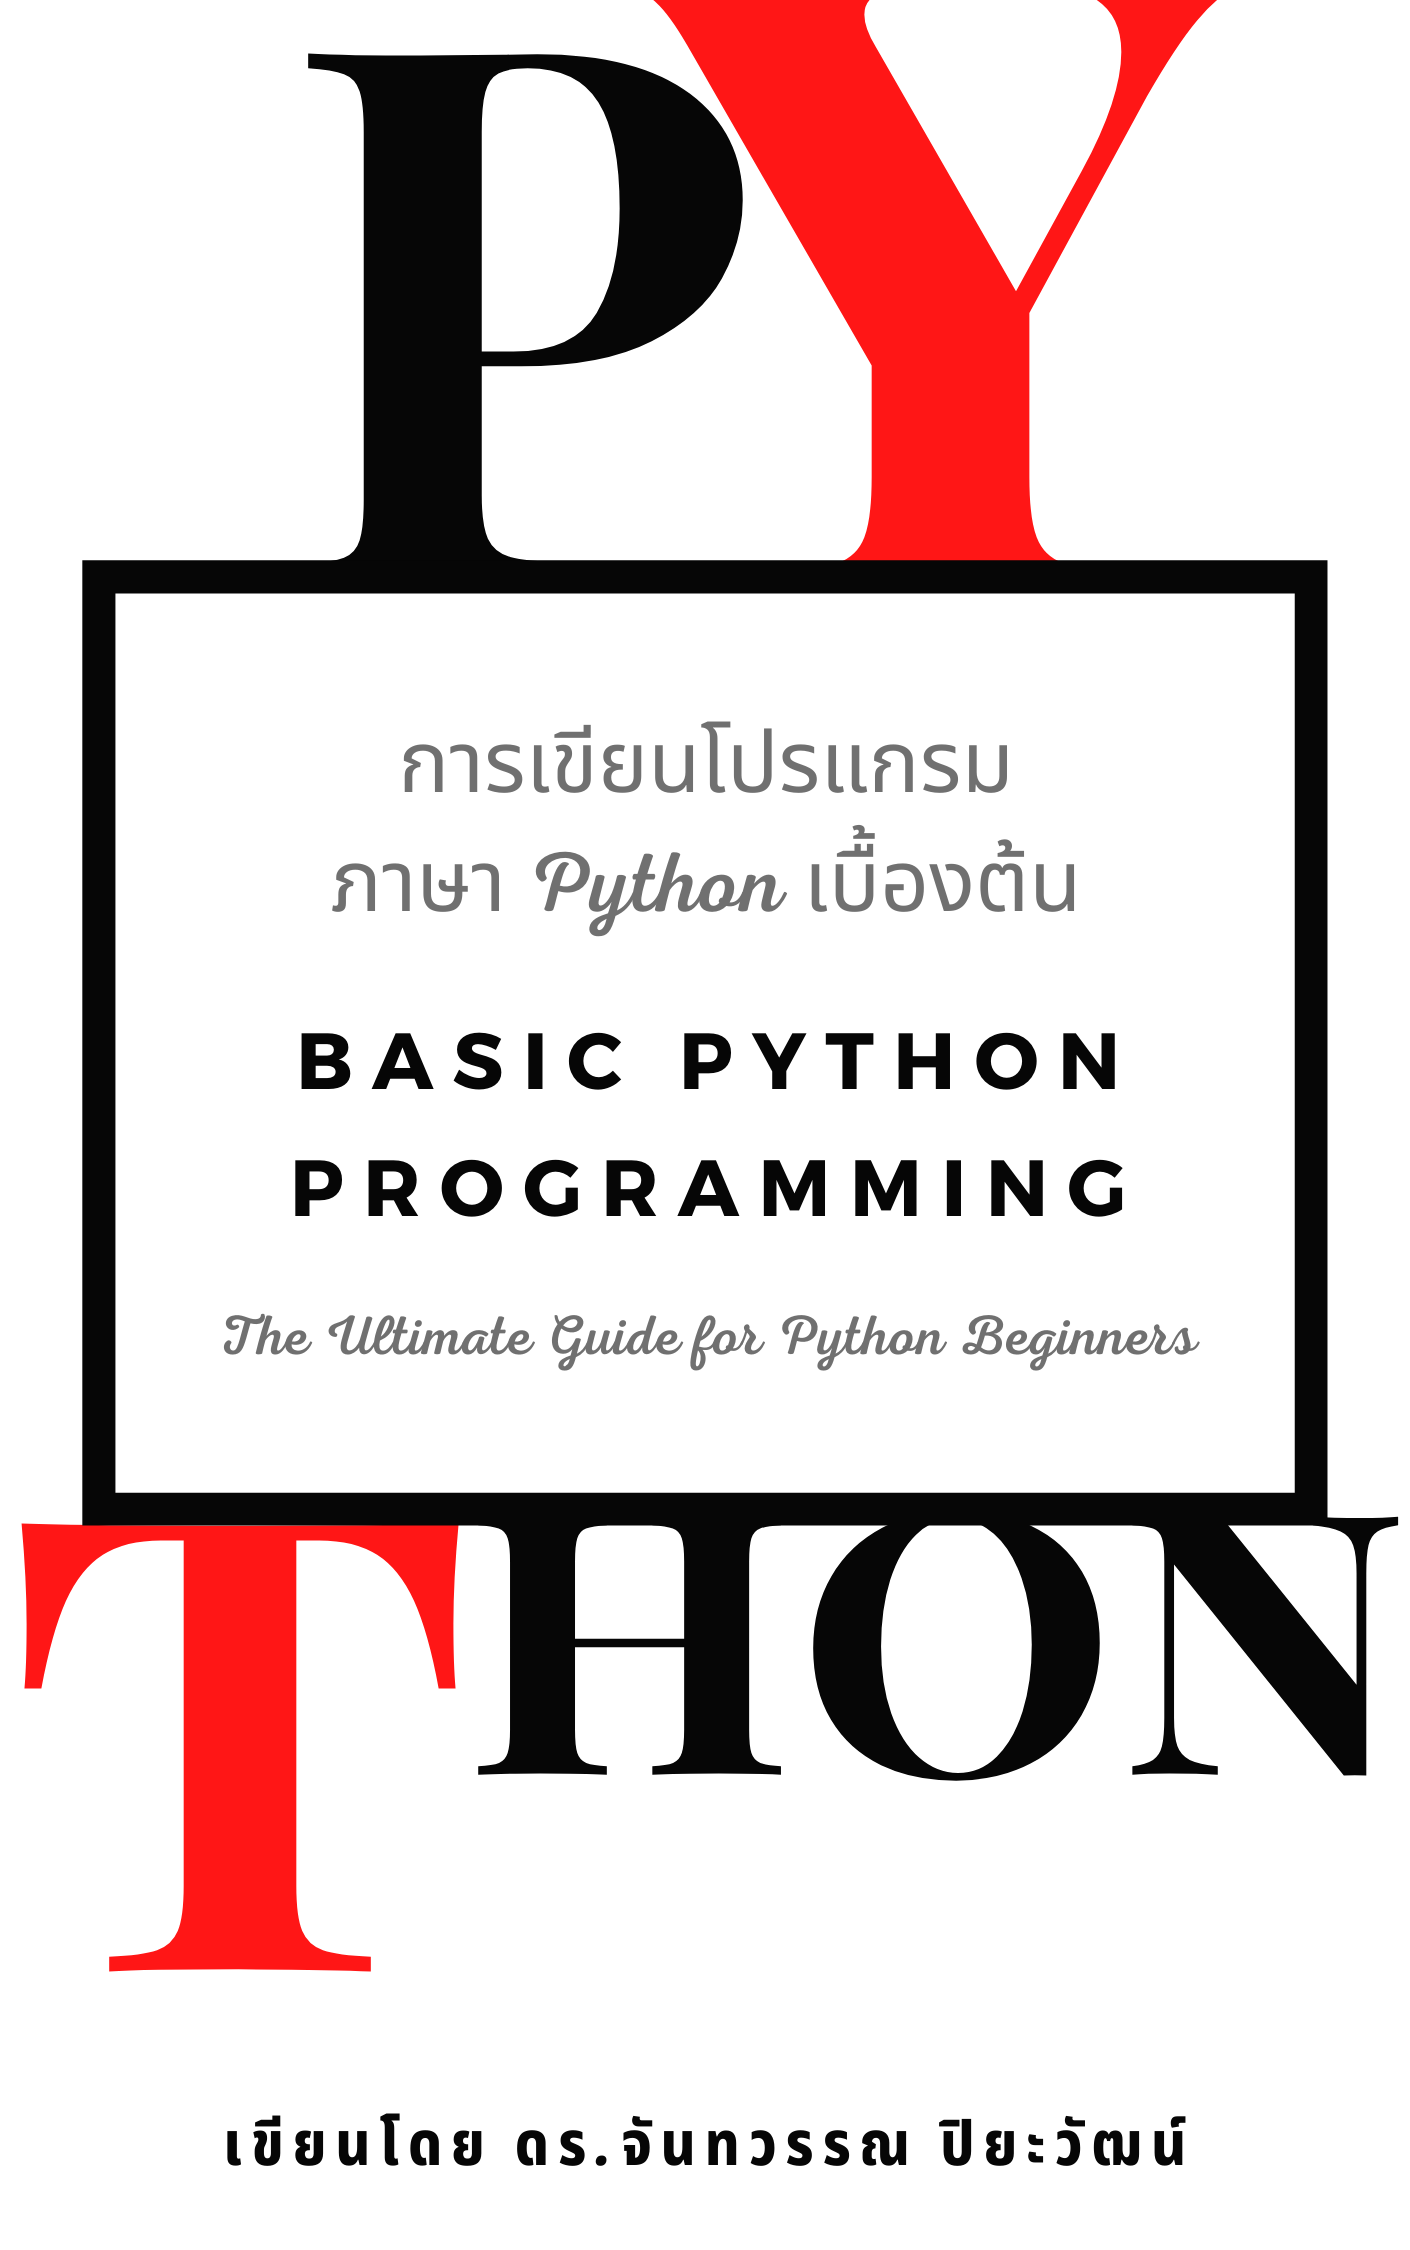
\includegraphics[width=\textwidth,height=23cm,keepaspectratio]{bookcover.png}
\end{titlepage}

\title{
477-201 การเขียนโปรแกรมคอมพิวเตอร์\\
\vspace{1mm}
การเขียนโปรแกรมภาษา Python เบื้องต้น\\
(Basic Python Programming)
}
\author{
ดร. จันทวรรณ ปิยะวัฒน์\\
\vspace{1mm}\\
สาขาวิชาระบบสารสนเทศทางธุรกิจ\\
ภาควิชาบริหารธุรกิจ คณะวิทยาการจัดการ\\
มหาวิทยาลัยสงขลานครินทร์\\
ภาคการศึกษาที่ 1/2563
}
\date{\vspace{1ex}}
\maketitle
\chapter{คำนำ}

\begin{markdown}

เอกสารประกอบการสอนเล่มนี้ จัดทำขึ้นสำหรับการสอนรายวิชา 477-201 การเขียนโปรแกรม คอมพิวเตอร์ (Computer Programming) ในภาคการศึกษาที่ 1 ปีการศึกษา 2562 ซึ่งเป็นรายวิชาบังคับของนักศึกษาหลักสูตรระบบสารสนเทศทางธุรกิจ ชั้นปีที่ 2 ภาควิชาบริหารธุรกิจ คณะวิทยาการจัดการ มหาวิทยาลัยสงขลานครินทร์ วิทยาเขตหาดใหญ่ จำนวน 3 หน่วยกิต 3(2-2-5) เป็นการสอนทฤษฎี 2 ชั่วโมงต่อสัปดาห์ ปฏิบัติ 2 ชั่วโมงต่อสัปดาห์ และนักศึกษาควรศึกษาค้นคว้าด้วยตัวเอง 5 ชั่วโมงต่อสัปดาห์

วิชา 477-201 การเขียนโปรแกรมคอมพิวเตอร์ มีจุดมุ่งหมายให้นักศึกษาได้มีพื้นฐาน ความรู้ความเข้าใจในหลักการเขียนโปรแกรมคอมพิวเตอร์เบื้องต้นด้วยภาษา Python ส่วนประกอบ ต่างๆของโปรแกรมคอมพิวเตอร์และภาษา Python สามารถเขียนโปรแกรมคอมพิวเตอร์พื้นฐาน ด้วยภาษา Python ได้ตามการวิเคราะห์และออกแบบขั้นตอนการทำงานของโปรแกรมอย่างมีระบบ สามารถเขียนโปรแกรมแบบมีเงื่อนไขเพื่อการตัดสินใจ เขียนคำสั่งเพื่อให้โปรแกรมทำงานวนซ้ำได้ และเข้าใจการใช้งานโมดูลส่วนเสริมต่างๆ ของโปรแกรมภาษา Python เพื่อนำความรู้เหล่านี้ไปใช้ ในการเขียนโปรแกรมระดับในระดับที่ยากขึ้น ซึ่งได้แก่ การเขียนโปรแกรมแบบฟังก์ชันและ การเขียนโปรแกรมเชิงวัตถุได้

หนังสือเล่มนี้ได้จัดแบ่งเนื้อหาออกเป็น 11 บท ในแต่ละบทจะมีแบบฝึกหัดท้ายบทเพื่อให้ผู้เรียน ได้ลองวิเคราะห์และออกแบบแนวทางแก้ไขปัญหาและพัฒนาออกมาเป็นโปรแกรมด้วยภาษา Python ที่ได้เรียนรู้ไปแล้วได้ ทั้งนี้ผู้จัดทำหวังเป็นอย่างยิ่งว่าเอกสารประกอบการสอนฉบับนี้จะให้ความรู้และเป็นประโยชน์แก่ผู้เรียนและผู้อ่านทุกๆ ท่าน เพื่อสร้างความรู้ความเข้าใจในการฝึกเขียนโปรแกรมคอมพิวเตอร์เบื้องต้นให้ดียิ่งขึ้น หากมีข้อเสนอแนะประการใด ผู้จัดทำขอรับไว้ด้วยความขอบพระคุณยิ่ง

\end{markdown}

\vspace{1cm}
\noindent
\textbf{ดร.จันทวรรณ ปิยะวัฒน์}\\
สาขาวิชาระบบสารสนเทศทางธุรกิจ\\
ภาควิชาบริหารธุรกิจ คณะวิทยาการจัดการ\\
มหาวิทยาลัยสงขลานครินทร์
\tableofcontents
\listoffigures
\listoftables

\chapter{แผนการสอน}
\section{คำอธิบายรายวิชาและวัตถุประสงค์ที่ระบุไว้ในหลักสูตร}

แนวความคิดเรื่องการเขียนโปรแกรม ขั้นตอนวิธีในการแก้ไขปัญหา การสร้างคำสั่งสำหรับเขียนขั้นตอนวิธีการ เขียนผังงาน นิพจน์ คำสั่งในการเขียนโปรแกรม หลักไวยากรณ์ของภาษาโปรแกรมระดับสูง การเขียนโปรแกรมสมัยใหม่ การทดสอบ การแก้ไขโปรแกรม การติดตั้ง และการเขียนเอกสารประกอบโปรแกรม

Concept of programming, algorithm to solve the problem, flowchart, expression and instruction, high-level language syntax, modern programming, testing, debugging, installation and software documentation

\section{วัตถุประสงค์ของวิชา}

มีจุดมุ่งหมายให้นักศึกษาได้มีพื้นฐานความรู้ความเข้าใจในหลักการเขียนโปรแกรมคอมพิวเตอร์เบื้องต้นด้วยภาษา Python ส่วนประกอบต่างๆ ของโปรแกรมคอมพิวเตอร์และภาษา Python สามารถเขียนโปรแกรมคอมพิวเตอร์อย่างง่ายด้วยภาษา Python ได้ตามการวิเคราะห์และออกแบบขั้นตอนการทำงานของโปรแกรมอย่างมีระบบ และมีความรู้ความเข้าใจในการเขียนโปรแกรมแบบมีเงื่อนไขเพื่อการตัดสินใจ การเขียนคำสั่งเพื่อการทำงานซ้ำ และโมดูลส่วนเสริมต่างๆ ของโปรแกรมภาษา Python เพื่อเรียนรู้เรื่องการเขียนโปรแกรมแบบฟังก์ชันและการเขียนโปรแกรมเชิงวัตถุได้

\section{เนื้อหาวิชา}

% \lesson command definition

\newcommand{\lesson}[3]{
\subsection{สัปดาห์ที่ {#1}}
%\begin{mdframed}
\begin{tcolorbox}[breakable,enhanced,fonttitle=\bfseries,title=สัปดาห์ที่ {#1}]
\begin{description}

\item[ผู้สอน] จันทวรรณ ปิยะวัฒน์
\item[จำนวนชั่วโมงบรรยาย] 2
\item[จำนวนชั่วโมงปฎิบัติ] 2
\item[หัวข้อ/รายละเอียด] \hfill \\
{#2}
\item[กิจกรรมการเรียนการสอน/สื่อที่ใช้] \hfill
\begin{itemize}[leftmargin=0pt]
{#3}
\end{itemize}

\end{description}
\end{tcolorbox}
%\end{mdframed}
}

% --

\lesson{1}
{
\underline{เค้าโครงวิชา}

\begin{itemize}
\item วัตถุประสงค์รายวิชา
\item รายละเอียดเนื้อหาวิชา
\item การวัดผลและการประเมินผล
\item เงื่อนไขและข้อตกลงอื่น
\item วิธีการเรียนการสอน
\item เว็บไซต์และหนังสืออ่านประกอบ
\end{itemize}

\underline{ระบบจัดการการเรียนรู้ (ClassStart.org)}
\begin{itemize}
\item ระบบในภาพรวม
\item การสมัครสมาชิก
\item การเข้าห้องเรียนออนไลน์ของรายวิชา
\item การใช้งานระบบ
\item การเข้าอ่านเอกสารการสอนและคลิป
\item การส่งแบบฝึกหัดทางออนไลน์
\item การทำข้อสอบออนไลน์
\item การตรวจสอบคะแนนเก็บ
\item การบันทึกการเรียนรู้ (Reflections)
\item การสื่อสารออนไลน์
\end{itemize}

\underline{เว็บไซต์ Code.org}
\begin{itemize}
\item การสมัครสมาชิก
\item ฝึกการเขียนโปรแกรมง่าย ๆ (Game-based Learning) แบบ Block-based Programming
\end{itemize}
}
{
\item บรรยาย
\item ปฎิบัติการใช้ระบบ ClassStart.org
\item ปฎิบัติการเขียนโปรแกรมทางออนไลน์ที่ Code.org
}

\lesson{2}{}{\item x}
\lesson{3}{}{\item x}
\lesson{4}{}{\item x}
\lesson{5}{}{\item x}
\lesson{6}{}{\item x}
\lesson{7}{}{\item x}
\lesson{8}{}{\item x}
\lesson{9}{}{\item x}
\lesson{10}{}{\item x}
\lesson{11}{}{\item x}
\lesson{12}{}{\item x}
\lesson{13}{}{\item x}
\lesson{14}{}{\item x}
\lesson{15}{}{\item x}


\mainmatter
\chapter{ความรู้เบื้องต้นเกี่ยวกับ Python}

\section{Python คืออะไร}

ในปี ค.ศ. 1980 Mr. Guido van Rossum ได้พัฒนาภาษาโปรแกรมมิ่งขึ้นมาและให้ชื่อว่าภาษา Python และเผยแพร่ให้ใช้งานสู่สาธารณชนในปี ค.ศ. 1991 (Guido, 2019) Python เป็นภาษาโปรแกรมคอมพิวเตอร์ระดับสูงซึ่งไวยากรณ์ของภาษาระดับสูงนี้จะใกล้เคียงคำในภาษาอังกฤษทั่วไป (Downey, 2015) Python ถูกใช้ในการสร้างโมบายแอพพลิเคชั่น เว็บไซต์ เว็บแอพพลิเคชั่น ออนไลน์เซอร์วิส รวมทั้งใช้ใน การวิเคราะห์ข้อมูลและคำนวณ ทางคณิตศาสตร์และวิทยาศาสตร์อย่างแพร่หลาย  ตัวอย่าง ออนไลน์เซอร์วิสที่พัฒนาขึ้นด้วยภาษา Python ได้แก่ Instagram, Uber, Pinterest, Reddit, Spotify และ Dropbox (Shuup, 2019) โดยในระยะหลายปี ที่ผ่านมานี้ Python ได้รับความนิยมสูงขึ้นเรื่อยๆ โดยในเดือนมิถุนายน 2562 ดัชนีความนิยมภาษาโปรแกรมมิ่ง TIOBE ได้แสดงให้เห็นว่า Python เป็นภาษาโปรแกรมมิ่ง ที่ได้รับความนิยมเป็นอันดับที่ 3 เทียบกับภาษาโปรแกรมมิ่งอื่นๆ และมีความนิยมสูงสุดในรอบ 19 ปี (TIOBE, 2019)

หากเปรียบเทียบกับภาษาโปรแกรมมิ่งอื่นๆ แล้ว Python มีไวยากรณ์ภาษา (Syntax) ที่สามารถอ่านง่าย เข้าใจได้ง่าย และเรียนรู้ง่าย Python จึงเป็นภาษาที่เหมาะสมสำหรับการสอนการเขียนโปรแกรมโดยเฉพาะอย่างยิ่งในระดับเบื้องต้น อีกทั้งยังเป็นภาษาที่ยืดหยุ่นสามารถพัฒนาได้บน ระบบปฏิบัติการที่หลากหลาย อาทิ  Windows, Linux, OS/2, MacOS, iOS และ Android นอกจากนี้ โปรแกรมเมอร์ทั่วโลกได้พัฒนาไลบรารี (Libraries) ขึ้นมาจำนวนมากสำหรับต่อยอด การทำงานของภาษา Python พื้นฐาน เช่น Django, Numpy, Pandas, Matplotlib, Flask, Web2py เป็นต้น (Foundation, 2019)

\section{Python ทำงานอย่างไร}

ภาษาโปรแกรมมิ่งระดับสูงจะต้องถูกโปรแกรมแปลภาษา เช่น คอมไพเลอร์ (Compiler) หรือ อินเทอร์พรีเตอร์ (Interpreter) ทำการแปลภาษาระดับสูงให้กลายเป็นภาษาเครื่องที่คอมพิวเตอร์เข้าใจก่อน (Lutz, 2013) ภาษาตระกูลที่ต้องใช้ Compiler เพื่อแปลงเป็นภาษาคอมพิวเตอร์ซึ่งเป็นภาษาที่มนุษย์อ่านไม่ออกแล้วจึงจะทำงานได้ เช่น ภาษา Java ภาษา C หรือภาษา C++ ภาษาพวกนี้จะได้โปรแกรมที่ทำงานรวดเร็วมาก แต่ก็ยากที่จะเรียนรู้ในช่วงการฝึกฝนการเขียน Programming ใหม่ๆ (Barry, 2016)

แต่สำหรับภาษา Python เมื่อได้ Source code ที่เป็นนามสกุลไฟล์ \texttt{.py} แล้ว โปรแกรมจะถูกคอมไพล์โดยคอมไพเลอร์ของ Python เพื่อแปลคำสั่ง Python ให้เป็นคำสั่งแบบ Bytecode และบันทึกไว้ในไฟล์นามสกุล \texttt{.pyc} ต่อมาเมื่อผู้ใช้ต้องการ Run ไฟล์นี้ อินเทอร์พรีเตอร์ (Interpreter) ก็จะแปลง Bytecode เป็นภาษาเครื่องสำหรับการดำเนินการโดยตรงบนฮาร์ดแวร์ (Beazley \& Jones, 2013) อาจเรียกได้ว่า Python เป็นภาษาลูกครึ่งและเรียนรู้ได้ง่าย เหตุผลที่ Python ทำการคอมไพล์เป็น Bytecode เป็นรหัสกลางไว้ก่อนนั้น นั่นก็เพราะ Python ถูกออกแบบมาให้เป็นภาษาการเขียนโปรแกรมที่ไม่ขึ้นกับแพลตฟอร์ม ซึ่งหมายความว่ามีการเขียนโปรแกรมหนึ่งครั้ง แต่สามารถเรียกใช้งานบนอุปกรณ์ใดก็ได้ แต่จะต้องติดตั้ง Python เวอร์ชันที่เหมาะสม 
\begin{markdown}

# ส่วนประกอบต่าง ๆ ของภาษา Python

## ตัวแปร (Variables)

ตัวแปร (Variables) คือชื่อที่กำหนดขึ้นสำหรับใช้เก็บค่าในหน่วยความจำของเครื่องคอมพิวเตอร์

## การตั้งชื่อตัวแปร

การตั้งชื่อตัวแปรมีเงื่อนไขดังนี้

1. ให้ขึ้นต้นด้วยอักษรตัวภาษาอังกฤษตัวใหญ่หรือตัวเล็กตั้งแต่ Aa ถึง Zz เท่านั้น 
1. ประกอบด้วยตัวอักษรหรือตัวเลข 0 ถึงเลข 9 หรือตัวขีดล่าง Underscore (_) แต่ห้ามมีช่องว่าง
1. ตัวเลข 0-9 จะนำหน้าชื่อตัวแปรไม่ได้
1. ตัวพิมพ์เล็กและตัวพิมพ์ใหญ่เป็นตัวแปรคนละตัวกัน (Case-Sensitive) เช่น Name ไม่ใช่ตัวแปรเดียวกันกับ name และจะใช้ใส่เครื่องหมาย = ในการตั้งตัวแปรหรือให้ค่าแก่ตัวแปร นอกจากนี้การตั้งชื่อตัวแปรควรตั้งอย่างสมเหตุสมผล อีกทั้ง ภาษา Python จะมีคำที่ถูกสงวนไว้ในการเขียนโปรแกรม หรือ Keywords ซึ่งห้ามนำมาใช้ในการตั้งชื่อตัวแปร ชื่อฟังก์ชัน หรือ ชื่อคลาส มีดังต่อไปนี้ $\cite{lutz2014}$


\end{markdown}

\cite{lutz2014}

%\begin{minted}{python}
\begin{pycode}
>>> a
1
>>> id(a)
1538021648
\end{pycode}
%\end{minted}
 \chapter {ประโยคเงื่อนไขในภาษา Python (Conditional Statements)}

\section{การเปรียบเทียบค่า (Boolean Expressions)}

Boolean Expressions คือ การดำเนินการเปรียบเทียบค่าเพื่อให้ได้ผลลัพธ์ออกมาเป็นถูก ( \texttt{True}) หากเงื่อนไขเป็นจริง หรือผลลัพธ์เป็นผิด ( \texttt{False}) หากเงื่อนไขเป็นเท็จหรือไม่เป็นจริง การเปรียบเทียบค่าใช้กับคำสั่งตรวจสอบเงื่อนไขการตัดสินใจ \texttt{if} และคำสั่งการทำงานวนซ้ำทั้ง \texttt{for} และ \texttt{while} เช่น ค่าของ x มากกว่าค่าของ y ใช่หรือไม่ ซึ่งผลลัพธ์จะออกมาเป็น True หรือ False โดยตัวดำเนินการเปรียบเทียบในภาษา Python ได้แสดงไว้ในตารางต่อไปนี้

\begin{table}[H]
\caption{ตัวดำเนินการเปรียบเทียบในภาษา Python}
\centering
\begin{tabu}{l l}
 \hline
 สัญลักษณ์ & ความหมาย  \\ [0.5ex] 
 \hline
x == y	& x เท่ากับ y \\
x != y	& x ไม่เท่ากับ y \\
x > y	& x มากกว่า y \\
x < y	& x น้อยกว่า y \\
x >= y & x มากกว่าหรือเท่ากับ y \\
x <= y & x น้อยกว่าหรือเท่ากับ y \\
\end{tabu}
\end{table}

ส่วนตัวอย่างการใช้สัญลักษณ์เปรียบเทียบค่าเป็นดังนี้

\begin{codelist}{ตัวอย่างการใช้สัญลักษณ์เปรียบเทียบค่า}{}
>>> a = 5
>>> b = 6
>>> a == b
False
>>> 5 > 6
False
>>> 5 < 6
True
>>> 5 >= 6
False
>>> print('5 == 5 :', 5 == 5)
5 == 5 : True
>>> print('12 >= 13.47 : ', 12 >= 13.47)
12 >= 13.47 : False
>>> 
\end{codelist}

\section{ตัวดำเนินการทางตรรกศาสตร์ (Logical Operators)}

การเปรียบเทียบค่ามากกว่าหนึ่งครั้งเชื่อมต่อกันสามารถดำเนินการได้โดยใช้ตัวดำเนินการทางตรรกศาสตร์ (Logical Operators) ในภาษา Python นั้นมีตัวดำเนินการทางตรรกศาสตร์ 3 ชนิด ซึ่งได้แก่ และ (\texttt{and}) หรือ (\texttt{or}) ไม่ (\texttt{not}) เช่น \texttt{a > 2 or c > b and c >2} ตัวอย่างการใช้ตัวดำเนินการทางตรรกศาสตร์ในภาษา Python เป็นดังต่อไปนี้

\begin{codelist}{ตัวอย่างการใช้ตัวดำเนินการทางตรรกศาสตร์ในภาษา Python}{}
>>> a = -4
>>> b = -2
>>> a > 2 or c > b and c> 2
False
\end{codelist}

ตัวดำเนินการทางตรรกศาสตร์  \texttt{and} ใช้เชื่อมสอง Expression ถ้าทั้งสอง Expression มีค่าเป็น True จะได้ผลลัพธ์เป็น \texttt{True}  ส่วนตัวดำเนินการทางตรรกศาสตร์ \texttt{or} ใช้เชื่อมสอง Expression ถ้าทั้งสอง Expression มีค่าเป็น False เท่านั้น ผลลัพธ์จึงจะเป็น \texttt{False} และตัวดำเนินการทางตรรกศาสตร์ \texttt{not} จะใช้ในการกลับค่าจาก \texttt{True} เป็น \texttt{False} และจาก \texttt{False} เป็น \texttt{True} ซึ่งผลการใช้ตัวดำเนินการทางตรรกศาสตร์ทั้งสามตัว แสดงไว้ในตารางดังต่อไปนี้

\begin{table}
\caption{ตารางผลการใช้ and}
\centering
\begin{tabu}{l l l}
 \hline
Boolean Expression 1 (BE1) & Boolean Expression 1 (BE2) & BE1 and BE2  \\ [0.5ex] 
 \hline
False & False & False \\
False & True & False  \\
True & False & False \\
\textbf{True} & \textbf{True} & \textbf{True} \\
\end{tabu}
\end{table}

\begin{table}
\caption{ตารางผลการใช้ or}
\centering
\begin{tabu}{l l l}
 \hline
Boolean Expression 1 (BE1) & Boolean Expression 1 (BE2) & BE1 or BE2  \\ [0.5ex] 
 \hline
\textbf{False} & \textbf{False} & \textbf{False} \\
False & True & True  \\
True & False & True \\
True & True & True \\
\end{tabu}
\end{table}

\begin{table}
\caption{ตารางผลการใช้ not}
\centering
\begin{tabu}{l l}
 \hline
 Boolean Expression & Not BE1  \\ [0.5ex] 
 \hline
False & True \\
True & False \\
\end{tabu}
\end{table}

\section{การใช้คำสั่ง \texttt{if} เพื่อเลือกเงื่อนไข}

เงื่อนไขที่ใช้ในภาษา Python คือ if Statement สิ่งที่ตามหลัง if คือ Boolean Expression เรียกว่า Statement ใหญ่ และใน Statement ใหญ่ ก็มี Statement ย่อย การดูว่า Statement ย่อยอยู่ใน if Statement ใดให้ดูที่การย่อหน้าหรือ Indentation ในภาษา Python การย่อหน้าสำคัญมากจะเป็นการบอกว่าอะไรอยู่ภายในอะไร 

รูปแบบของการใช้งานคำสั่ง if ในภาษา Python โดยถ้าหากเงื่อนไขเป็นจริง ตัวโปรแกรมจะประมวลผลในคำสั่ง if หลังเครื่องหมาย :  ดังต่อไปนี้

\begin{codelist}{รูปแบบของการใช้งานคำสั่ง if}{}
if expresion:
    #statements
\end{codelist}

ตัวอย่างเช่น ให้แสดงข้อความว่า อายุต่ำกว่าเกณฑ์ ถ้าหากค่าอายุที่รับเข้ามาต่ำกว่า 18 ปี การเขียน Source Code และผลลัพธ์ของโจทย์เป็นดังนี้ 

\begin{codelist}{ตัวอย่างการใช้ \texttt{if}}{}
age = int(input('Enter your age: `))
if age < 18:
   print('You are underage.')
\end{codelist}

\begin{codelist}{ผลลัพธ์จากโจทย์ตัวอย่างการใช้ \texttt{if}}{}
>>>
Enter your age: 15
You are underage.
>>>
\end{codelist}


\section{การใช้ \texttt{if} กับ \texttt{else}}

โครงสร้างคำสั่ง if…else จะดำเนินในบล็อคคำสั่ง else ถ้าหากเงื่อนไขในคำสั่ง if นั้นเป็นเท็จ โดยมีรูปแบบการเขียนดังนี้

\begin{codelist}{รูปแบบของการใช้งานคำสั่ง if-else}{}
if expression:
    # statements
else:
    # statements
\end{codelist}

ตัวอย่างการใช้ \texttt{if...else} และผลลัพธ์เป็นดังต่อไปนี้

\begin{codelist}{ตัวอย่างการใช้ \texttt{if...else}}{}
x = 15
y = 6
if x > y: print('x is greater than y.')
else: print('x is less than or equal to y.')
\end{codelist}


\begin{codelist}{ผลลัพธ์จากตัวอย่างการใช้ \texttt{if...else}}{}
>>>
x is greater than y.
>>>
\end{codelist}


\section{Chained Expressions}

การใช้ Chained Expressions คือ การใส่ elif ไปเรื่อยๆ และเงื่อนไขสุดท้ายจะต้องใช้ else โดยไม่ต้องการระบุ Boolean Expressions ใดๆ อีกแล้วหลังจากที่ใส่ else ดังตัวอย่างและผลลัพธ์ดังต่อไปนี้

\begin{codelist}{ตัวอย่างการเขียน Chained Expressions}{}
x = 6
y = 6
if x > y: print('x is greater than y.')
elif x < y: print('x is less than y.')
else: print('x and y are equal.')
\end{codelist}


\begin{codelist}{ผลลัพธ์ตัวอย่างการเขียน Chained Expressions}{}
>>>
x and y are equal.
>>>
\end{codelist}


\section{Nested Expressions}

if มี Statement อยู่ข้างในได้ และ else ก็มี Statement อยู่ข้างในได้เช่นกัน เรียกว่า Nested Expressions ดังตัวอย่างและผลลัพธ์ดังต่อไปนี้

\begin{codelist}{ตัวอย่างการเขียน Nested Expressions}{}
x = 7
y = 6
if x == y: print('x and y are equal.')
else:
    if x < y: print('x is less than y.')
    else: print('x is greater than y.')
\end{codelist}

\begin{codelist}{ผลลัพธ์ตัวอย่างการเขียน Nested Expressions}{}
>>>
x is greater than y.
>>>
\end{codelist}

\section{แบบฝึกหัด}

\begin{enumerate} 
\item  จงเขียน code ต่อไปนี้
\begin{itemize}
\item ให้ถามว่า Are you bored? และให้ตอบว่า y หรือ n
\item ถ้าตอบ y ให้พิมพ์ข้อความว่า Let’s go outside.
\end{itemize}
\item จงเขียน code ต่อไปนี้
\begin{itemize}
\item ตั้งค่าตัวแปร var รับค่าเป็นตัวเลขจำนวนเต็มจากผู้ใช้
\item ถ้า var > 100 ให้แสดงผลว่า “The value is over 100.”
\item ถ้า เป็นกรณีอื่นๆ ให้แสดงผลว่า “The value is less than or equal 100.”
\end{itemize}
\item จงเขียน code ต่อไปนี้
\begin{itemize}
\item รับค่า a, b เป็นจำนวนเต็ม
\item แสดงผลว่า a > b หรือ a < b หรือ a = b
\end{itemize}
\item จงเขียน code ต่อไปนี้
\begin{itemize}
\item รับค่า score เป็นจุดทศนิยม
\item ถ้าคะแนน 81-100 แสดงผลว่า เกรด A
\item ถ้าคะแนน 61-80  แสดงผลว่า เกรด B
\item ถ้าคะแนน 41-60 แสดงผลว่า เกรด C
\item ถ้าคะแนน 0-40 แสดงผลว่า เกรด F
\item เมื่อแสดงผลดังกล่าวแล้ว ให้แจ้งด้วยว่า “ตัดเกรดแล้ว”
\end{itemize}
\end{enumerate}

\chapter{การเขียนและใช้งานฟังก์ชัน (Functions)}
\section{การเรียกใช้ฟังก์ชัน}

ฟังก์ชัน (Function) คือชุดคำสั่งส่วนหนึ่งของโปรแกรมที่ทำงานเพื่อวัตถุประสงค์เฉพาะอย่าง ฟังก์ชันในภาษา Python มีทั้ง Built-in ฟังก์ชันของภาษา Python เอง และฟังก์ชันที่ผู้เขียนโปรแกรมเขียนขึ้นมา การใช้ฟังก์ชันในภาษา Python จะคล้ายกับฟังก์ชันทางคณิตศาสตร์ คือ กำหนดชื่อฟังก์ชันตามด้วยสิ่งที่อยู่ในวงเล็บซึ่งเรียกว่า Arguments ซึ่งอาจจะมีได้มากกว่า 1 และในภาษา Python มีการกำหนดฟังก์ชันมาให้เรียกใช้ได้เลยอยู่บ้างแล้ว เช่น \texttt{type(42)} คือ การแสดงค่าประเภทของเลข 42 หรือ \texttt{id(42)} คือการแสดงตำแหน่งที่อยู่ของเลข 42 ในหน่วยความจำ ดังตัวอย่างต่อไปนี้

\begin{codelist}{ตัวอย่าง Built-in ฟังก์ชันในภาษา Python}{}
>>> type(42)
|<class \rq{}int\rq{}>|
>>> a = 1
>>> id(a)
1538021648
\end{codelist}


\section{การเรียกใช้โมดูล (Modules)}

โมดูล (Modules) คือ ฟังก์ชันที่รวมกันไว้เป็นหมวดหมู่ และสามารถดึงมาใช้ได้ในโปรแกรมได้ด้วยการ \texttt{import} เช่น \texttt{import math} และหากเรียกใช้ฟังก์ชัน \texttt{dir(math)} จะแสดงฟังก์ชันในโมดูล math ออกมา ดังตัวอย่างต่อไปนี้

\begin{codelist}{การเรียกใช้โมดูล math}{}
>>> import math
>>> type(math)
|<class \rq{}module\rq{}>|
>>> id(math)
56337632

\end{codelist}


การใช้งานโมดูลจะมีการใช้งานแบบ Dot Notation หากเห็นการเขียนโมดูล math ในลักษณะนี้ เช่น  \texttt{math.pi} ตัว  \texttt{pi} เรียกว่าเป็นตัวแปรที่อยู่ในโมดูล  \texttt{math} ซึ่งไม่ใช่ฟังก์ชัน แต่ถ้าเขียน  \texttt{math.pow(2,2)} คือ สองยกกำลังสอง ลักษณะนี้จะเป็นการเรียกใช้ฟังก์ชันที่อยู่ในโมดูล ดังตัวอย่างต่อไปนี้

\begin{codelist}{การใช้งานโมดูลแบบ Dot Notation}{}
>>> math.pi
3.141592653589793
>>> math.pow(2,2)
4.0
\end{codelist}

%\section{ฟังก์ชันซ้อน (Composition)}
การใช้ฟังก์ชันไม่จำเป็นต้องใช้ฟังก์ชันแบบฟังก์ชันเดียว ฟังก์ชันใช้ฟังก์ชันซ้อนกันได้ คือ การรวมฟังก์ชันหลายๆ อันซ้อนกัน เรียกต่อๆ กันไปได้ ดังตัวอย่างต่อไปนี้

\begin{codelist}{การเรียกใช้ฟังก์ชันแบบ Composition}{}
>>> math.exp(math.log(3+2))
4.9999999999999
\end{codelist}

\section{การสร้างฟังก์ชันในภาษา Python}

การเขียนฟังก์ชันหรือสร้างฟังก์ชันขึ้นมาเองจะกระทำเพื่อต้องการให้โปรแกรมที่เขียนขึ้นมาทำงานเพื่อวัตถุประสงค์เฉพาะอย่าง ต้องใช้ \texttt{def} Statement ซึ่งย่อมาจาก Define เมื่อเขียนฟังก์ชันไว้ใน Source Code แล้วทำการ Run ฟังก์ชันนั้นจะถูก Define ไว้ในระบบแล้วถูกเรียกใช้ขึ้นมาได้เลย ด้วยการเรียกชื่อฟังก์ชันนั้นกี่ครั้งต่อกี่ครั้งก็ได้ ดังรูปแบบการเขียนต่อไปนี้ทั้งในแบบที่มีการคืนค่าและไม่มีการคืนค่า

\begin{codelist}{รูปแบบการสร้างฟังก์ชัน}{}
def function_name(args...):
    # statements

def function_name(args...):
    # statements
    return value
\end{codelist}

ส่วนวิธีการเรียกใช้ฟังก์ชันทำได้โดย เรียกชื่อฟังก์ชันนั้นตามด้วยวงเล็บ () ซึ่งจะมี Arguments หรือไม่ก็แล้วแต่ฟังก์ชันที่กำหนดไว้ ดังตัวอย่างการเรียกใช้ฟังก์ชันที่สร้างขึ้นมาเองต่อไปนี้

\begin{codelist}{ตัวอย่างฟังก์ชันที่สร้างขึ้นมาเอง}{}
def happy_birthday_song():
    print('Happy Birthday.')
    print('Happy Birthday to you.')
\end{codelist}

\begin{codelist}{ผลลัพธ์จากตัวอย่างการเรียกใช้ฟังก์ชันที่สร้างขึ้นมาเอง}{}
>>>  happy_birthday_song()
Happy Birthday.
Happy Birthday to you.
\end{codelist}


\section{ขอบเขตของตัวแปร}

ในวงเล็บ () เป็นการกำหนด Argument ของฟังก์ชัน ซึ่งจะกลายเป็นพารามิเตอร์ (Parameters) หรือตัวแปรที่ใช้ในฟังก์ชันนั้นๆ เท่านั้นและต้องประมวลผลให้เสร็จสิ้นในฟังก์ชัน หรือเรียกว่า Local Variables ตัวแปร Local นี้ จะไม่สามารถเรียกใช้ที่โปรแกรมหลักได้ และผู้เขียนโปรแกรมก็ไม่สามารถนำตัวแปรนี้ไปใช้ในฟังก์ชันอื่น ๆ ได้ ส่วนตัวแปร Global (Global Variables) จะประกาศไว้ในส่วนหลักของโปรแกรมที่เขียนขึ้น ฟังก์ชันย่อยและตัวโปรแกรมหลักสามารถเรียกใช้ตัวแปร Global ได้

\begin{codelist}{ตัวอย่างการใช้ Local และ Global Variables}{}
def newage(age):
    a = 50 #local variable
    x = age + a #local variable
    return x

age = int(input('Enter your age: ')) #global variable
print('In 50 years from now, you will be ', newage(age), end='.')
\end{codelist}

\begin{codelist}{ผลลัพธ์ตัวอย่างการใช้ Local และ Global Variables}{}
Enter your age: 18
In 50 years from now, you will be  68.
>>> 
\end{codelist}


ตัวแปรใดก็ตามที่จะใช้เป็น Local ให้ใส่คำว่า \texttt{global} ไปด้านหน้าตัวแปรที่ถูกเรียกใช้ในฟังก์ชัน อันที่จริงแล้วจะไม่เขียนคำว่า \texttt{global}  ก็ได้หากชื่อตัวแปรไม่ซ้ำกันเลย

\begin{codelist}{ตัวอย่างการใช้ Global Variables}{}
x = 5
def happy_birthday_song(name):
    global x
    print('Happy Birthday.')
    print('Happy Birthday.')
    print('Happy Birthday.')
    print('Happy Birthday to ' , name)
    print(x)
happy_birthday_song('Mike')
\end{codelist}

\begin{codelist}{ผลลัพธ์ตัวอย่างการใช้ Global Variables}{}
>>>
Happy Birthday.
Happy Birthday.
Happy Birthday.
Happy Birthday to Mike
5
>>>
\end{codelist}

\section{ฟังก์ชัน \texttt{return}}

ฟังก์ชันทุกอันจะต้อง return คือสิ้นสุดการทำงาน แต่ได้เว้นไว้ในฐานที่เข้าใจ เมื่อโปรแกรมไล่การทำงานมาถึงจุด return โปรแกรมจะหยุดทำงานทันทีทั้งๆ ที่ยังมีคำสั่งอื่นตามมาหลังจาก return อีกก็ตาม  ฟังก์ชัน \texttt{return} ซึ่งไม่ได้คืน ค่าอะไรออกมาเรียกว่า Void 

\begin{codelist}{ตัวอย่างการใช้ \texttt{return}}{}
x = 5
def happy_birthday_song(name):
    print('Happy Birthday.')
    return
    print('Happy Birthday.')
    print('Happy Birthday.')
    print('Happy Birthday to ' , name)
    print(x)
happy_birthday_song('Mike')
\end{codelist}

\begin{codelist}{ผลลัพธ์ตัวอย่างการใช้ \texttt{return}}{}
>>>
Happy Birthday.
>>>
\end{codelist}

\section{การคืนค่าจากฟังก์ชัน}

ฟังก์ชันสามารถ return ค่าได้ด้วย ดังเช่นตัวอย่างการหาพื้นที่สี่เหลี่ยม โดยกำหนดฟังก์ชันชื่อ \\  \pyinline{rectangle_area(width, height)} และฟังก์ชันมีพารามิเตอร์สองตัวสำหรับความกว้างและความยาวของสี่เหลี่ยม และฟังก์ชันทำการคืนค่า ผลลัพธ์ที่เป็นพื้นที่กลับไปด้วยคำสั่ง \pyinline{return}

ตัวอย่างการหาพื้นที่สี่เหลี่ยม  เป็นดังต่อไปนี้

\begin{codelist}{ตัวอย่างการใช้ \texttt{return} ที่มีการส่งค่ากลับ}{}

def happy_birthday_song(name):
    print('Happy Birthday.')
    print('Happy Birthday.')
    print('Happy Birthday.')
    print('Happy Birthday to ' , name)
    return name

def rectangle_area(width, height):
    return width * height  #การส่งค่ากลับ
    
x = rectangle_area(4, 3)
print('The area of rectangle is', str(x))
\end{codelist}

ผลลัพธ์ของตัวอย่างการหาพื้นที่สี่เหลี่ยม เป็นดังต่อไปนี้

\begin{codelist}{ผลลัพธ์ตัวอย่างการใช้ \texttt{return} ที่มีการส่งค่ากลับ}{}
>>>
The area of rectangle is 12
>>>
\end{codelist}


อีกตัวอย่างของฟังก์ชันที่สร้างขึ้นมาเองโดยมีการใช้ return

\begin{codelist}{ตัวอย่างฟังก์ชันที่สร้างขึ้นมาเองโดยมีการใช้ return}{}
def newage(age):
    x = age+50
    return x #การส่งค่ากลับ

age = int(input('Enter your age: '))
print('In 50 years from now, you will be ', newage(age), end='.')
\end{codelist}

ผลลัพธ์จากตัวอย่างฟังก์ชันที่สร้างขึ้นมาเองโดยมีการใช้ return เป็นดังต่อไปนี้

\begin{codelist}{ผลลัพธ์จากตัวอย่างฟังก์ชันที่สร้างขึ้นมาเองโดยมีการใช้ return}{}
>>>
Enter your age: 6
In 50 years from now, you will be  56.
>>> 
\end{codelist}

\section{การเขียนโปรแกรมเชิงฟังก์ชัน (Functional Programming)}


การเขียนโปรแกรมเชิงฟังก์ชัน (Functional Programming) เป็นรูปแบบการเขียนโปรแกรมที่เก่าแก่ที่สุดและเป็นรูปแบบที่กลับมาได้รับความนิยมมากในปัจจุบัน คือสร้างฟังก์ชันแล้วให้ฟังก์ชันทำงานร่วมกันโดยไม่มีการใช้ Global Variables เลย ฟังก์ชันหนึ่งทำงานส่งผลลัพธ์แก่อีกฟังก์ชันหนึ่งต่อๆ กันไปเรื่อยๆ ซึ่งภาษา Python สามารถใช้เขียนโปรแกรมแบบนี้ได้ ฟังก์ชันแล้ว return ค่าเป็นผลลัพธ์แก่อีกฟังก์ชันหนึ่งไปเรื่อยๆ  

จากรูป  \pyinline{x=f(g(h(x)))} ทำงานเหมือนกันกับ  \pyinline{x = h(x) }แล้ว  \pyinline{x = g(x)} แล้ว  \pyinline{x = f(x)}

\begin{codelist}{Functional Programming}{}
x = f(g(h(x)))
x = h(x)
x = g(x)
x = f(x)
\end{codelist}


\section{ฟังก์ชันที่เรียกตัวเอง (Recursion)}

Recursion คือการเรียกใช้ฟังก์ชันซ้อนฟังก์ชันนั้นๆ เอง หรือ ฟังก์ชันเรียกใช้ตัวมันเอง จากฟังก์ชัน  \pyinline{countdown()} ในตัวอย่าง เมื่อมีการเรียกฟังก์ชัน  \pyinline{countdown(5)} โปรแกรมจะทำงานลดหลั่นลงไปเรื่อยๆ คือตั้งแต่ 5, 4, 3, 2, 1 ตราบเท่าที่ n ยังมากกว่า 0 แต่เมื่อเงื่อนไขเป็นเท็จแล้ว โปรแกรมจะแสดงคำว่า Go! แทน ซึ่งมีลักษณะการเขียนดังนี้


\begin{codelist}{ตัวอย่างการใช้ Recursion}{}
def countdown(n):
    if x > 0:
        print(n)
        countdown(n-1)
    else:
        print('Go.')
\end{codelist}

ซึ่งจะได้ผลลัพธ์ดังนี้
\begin{codelist}{ผลลัพธ์จากตัวอย่างการใช้ Recursion}{}
>>> countdown(5)
5
4
3
2
1
Go.
\end{codelist}

\begin{enumerate} 

\section{แบบฝึกหัด}

\item ตั้งชื่อฟังก์ชัน \pyinline{hello} เพื่อแสดงผลว่า สวัสดีคุณ
\item สร้างฟังก์ชันคำนวณพื้นที่ รับค่า ความกว้าง และ ความยาว
\item สร้างฟังก์ชันชื่อ  \pyinline{maximal_2} รับ arguments 2 ค่า และ return ค่าที่มากที่สุดออกมา
\item สร้างฟังก์ชันชื่อ  \pyinline{maximal_3} รับ arguments 3 ค่า และ return ค่าที่มากที่สุดออกมา
\item สร้างฟังก์ชันรับ arguments 3 ค่า และ return ผลคูณออกมา
\item สร้างฟังก์ชันรับค่าตัวเลขในหน่วยเมตรต่อวินาที แล้ว return ผลในหน่วยกิโลเมตรต่อชั่วโมง
\item สร้างฟังก์ชันหาผลต่างของรายรับกับรายจ่าย และส่งผลกลับมา

\end{enumerate}



\chapter{การใช้ประโยคสั่งทำงานวนซ้ำ}
\section{ฟังก์ชัน range()}

ฟังก์ชัน range() คือ ระยะตั้งแต่เริ่มต้นถึงก่อนระยะสิ้นสุด มักจะใช้ในการควบคุมการทำงานของโปรแกรมเป็นจำนวนรอบ มีวิธีการเขียนดังนี้ range(start, end)

\section{คำสั่ง for}

คำสั่ง for statement เป็นการทำงานซ้ำๆ ตามจำนวนครั้งที่ระบุไว้ เช่น การใช้ for statement ร่วมกัน range() โดยมีรูปแบบการเขียนดังนี้


\section{คำสั่ง while}

while Statement เป็นคำสั่งให้โปรแกรมทำงานวนซ้ำในขณะที่เงื่อนไขของการวนซ้ำนั้นยังคงเป็นจริงอยู่ และเมื่อเงื่อนไขเป็นเท็จจะสิ้นสุดการทำงานวนซ้ำนั้นทันที ดังนั้นจึงต้องมีตัวควบคุมในการเพิ่มค่าไปเรื่อยๆ จนเงื่อนไขเป็นเท็จ มีลักษณะการเขียนดังนี้


\section{คำสั่ง break}

คำสั่ง break เพื่อให้หลุดการทำงานในลูป

\section{ฟังก์ชันที่เรียกตัวเอง (Recursion)}

Recursion คือการเรียกใช้ฟังก์ชันซ้อนฟังก์ชันนั้นๆ เอง หรือ ฟังก์ชันเรียกใช้ตัวมันเอง จากฟังก์ชัน countdown() ในตัวอย่าง เมื่อมีการเรียกฟังก์ชัน countdown(5) โปรแกรมจะทำงานลดหลั่นลงไปเรื่อยๆ คือตั้งแต่ 5, 4, 3, 2, 1 ตราบเท่าที่ n ยังมากกว่า 0 แต่เมื่อเงื่อนไขเป็นเท็จแล้ว โปรแกรมจะแสดงคำว่า Go! แทน


\section{แบบฝึกหัด}
\begin{enumerate} 

\item 	สร้างฟังก์ชันหาค่าของ \pyinline{ \[ 3^1 + 3^2 + 3^3 + 3^4 + 3^5 \] } โดยใช้ For loop
\item 	สร้างฟังก์ชันให้ผู้ใช้ป้อนค่า x แล้วนำค่า x มาคำนวณ \pyinline{x^1+x^2+x^3+x^4+x^5}
\item 	สร้างฟังก์ชันให้ผู้ใช้ป้อนค่า n และให้แสดงเลขเริ่มที่ n โดยลดลงทีละหนึ่ง โดยใช้ While loop
\item 	สร้างฟังก์ชันให้ผู้ใช้ป้อนตัวเลข แล้วหาว่ามีเลขใดที่สามารถหารเลขที่ผู้ใช้ป้อนได้ลงตัว เช่น ผู้ใช้ป้อนตัวเลข 4 จะมี 1 2 4 ที่หารเลข 4 ลงตัว
\item 	สร้างฟังก์ชันคำนวณปีเกิด คศ. เป็น 12 ราศีปีนักษัตร
\item 	สร้างฟังก์ชันรับจำนวนเงินมาหนึ่งค่า แล้วแลกเปลี่ยนธนบัตร 100 บาท 50 บาท 20 บาท เหรียญ 10 บาท 5 บาท และ 1 บาท
\end{enumerate}
\chapter{การใช้งาน String}
\section{ความหมายของ String}

String คือ ข้อความหรือตัวอักษรที่เรียงต่อๆ กันที่อยู่ในเครื่องหมายคำพูดแบบ Double Quotes เช่น “How are you?” หรือ Single Quotes เช่น ‘How are you?’ 

\section{ฟังก์ชัน \texttt{len()}}

มีฟังก์ชันสำหรับ String อยู่หลายฟังก์ชัน เช่น ฟังก์ชัน \pyinline{len()} มีวัตถุประสงค์เพื่อหาความยาวของ String นั้น และสำหรับการระบุตำแหน่งของตัวอักษรแต่ละตัวใน String จะใช้สัญลักษณ์ก้ามปู \pyinline{[ ]} โดยตัวชี้หรือ Index จะเริ่มต้นจาก 0 เช่น \pyinline{fruit[0]}

\section{การเดินทางตามตัวชี้ของ String}

การเดินทางไปเรื่อยๆ ตามตัวชี้ของ String โดยในตัวอย่างแรกจะเป็นการใช้ while ส่วนในตัวอย่างถัดมาจะใช้ตัวแปร string เป็น Iterator ซึ่งผลลัพธ์จะออกมาเหมือนกัน


\section{การตัดคำใน String}

การตัดคำใน String ด้วยตัวชี้ (Index) โดยการตัดคำเป็นส่วนย่อยๆ จะมีรูปแบบการเขียนเป็น [start:end] โดยที่ start เป็นตำแหน่งของ Index เริ่มต้นที่ต้องการ และ end นั้นเป็นตำแหน่งก่อนหน้าตำแหน่งสุดท้ายของตัวอักษรที่ต้องการ 

หากเขียนเป็น [start:] ระบุจุดเริ่มต้นที่ start ผลลัพธ์จะแสดงยาวไปจนถึงจุดสิ้นสุด และหากเขียนเป็น [:end] ผลลัพธ์ที่ได้จะแสดงอักษรตั้งแต่ตัวแรกหรือตัวชี้ที่ศูนย์ไปจนถึงตัวสิ้นสุดที่ระบุไว้

\section{โครงสร้างข้อมูลที่เปลี่ยนแปลงไม่ได้}

String เป็นโครงสร้างข้อมูลที่เปลี่ยนแปลงไม่ได้ ดังนั้นถ้าหากต้องการสร้าง String ใหม่ก็ต้องสร้างเป็น Object ใหม่เท่านั้น

\section{การค้นหาตัวอักษรใน String}

การเขียนโปรแกรมเพื่อค้นหาตัวอักษรใน String แล้วส่งค่าออกมาเป็นค่าตัวชี้ตัวอักษรใน String สามารถเขียนเป็นตัวอย่างฟังก์ชันดังนี้ คือ 

\begin{itemize}
\item ให้ฟังก์ชันชื่อว่า find มีการส่งค่า str เป็น string และค่า char เป็น character 
\item ตั้งตัวนับ i เริ่มต้นที่ 0
\item ขณะที่ i ยังน้อยกว่าจำนวนตัวอักษรใน string ที่ชื่อว่า str ให้ดำเนินการดังนี้คือ
	\begin{itemize}
		\item ตรวจสอบว่า ถ้าตัวชี้ของตัวอักษรเท่ากับตัวอักษรที่ต้องการแล้ว ให้ส่งค่าตัวนับออกมา
	\end{itemize}
\item เมื่อ while เป็นเท็จแล้ว หรือเมื่อค้นจนครบ character ใน string แล้วให้ส่งค่ากลับคือ -1
\end{itemize}

\section{เมธอดของ String (String Methods)}

การดำเนินการกับ String สามารถศึกษาฟังก์ชันได้ที่ \url{https://docs.python.org/2.4/lib/string-methods.html} เช่น str.upper() ใช้ทำงานเพื่อแปลงตัวอักษรภาษาอังกฤษเป็นตัวพิมพ์ใหญ่

\section{\texttt{in} โอเปอร์เรเตอร์}

ใช้ในการพิสูจน์ค่าแบบ Boolean Expression เช่น ‘t’ in s แปลว่า ตัวอักษรตัว t อยู่ใน string ชื่อว่า s หรือไม่ หรือในทางตรงข้ามเพื่อการตรวจสอบว่าไม่มีหรือไม่ให้ใส่ not in 

\section{การเปรียบเทียบ String}

การเปรียบเทียบ String สามารถใช้สัญลักษณ์  ( > , < , <= , <= , == , !=  ) เพื่อเปรียบเทียบค่าของ String สองชุด โดยดูผลลัพธ์ของการเปรียบเทียบค่าของ ASCII value นั้นๆ

\section{การจัดวางรูปแบบของ String (String Formatting)}

การเปลี่ยนการจัดวางรูปแบบของ String มีสองวิธีคือ แบบ Classic ซึ่งทำได้โดยใส่สัญลักษณ์ + แต่สัญลักษณ์นี้จะมีข้อจำกัดคือไม่สามารถแทรกข้อความระหว่างกันได้ แต่หากใช้สัญลักษณ์ \% จะช่วยแก้ไขข้อจำกัดนี้ได้ เช่น \%s สำหรับ string และ \%d สำหรับตัวเลข 

ส่วนการเปลี่ยนการจัดวางของ String แบบ Modern คือ ใช้ .format และระบุ Parameters ได้มากกว่า 1 ตัว อีกทั้งยังสามารถจัดเรียงลำดับ Parameters สลับก่อนหลังได้ตามสะดวก สามารถศึกษาเพิ่มเติมได้ที่ \url{https://docs.python.org/3/library/string.html\#format-examples}

\section{แบบฝึกหัด}
\begin{enumerate} 
\item 	เขียนฟังก์ชันต่อไปนี้
\begin{itemize}
\item 	รับค่าข้อความ “James had had had the cat.”
\item 	นับจำนวนคำว่า had
\end{itemize}
\item 	เขียนฟังก์ชันต่อไปนี้
\begin{itemize}
\item 	รับค่าข้อความ “I intend to live forever, or die trying.”
\item 	แทนค่าคำว่า to ด้วย three
\end{itemize}
\item 	เขียนฟังก์ชันต่อไปนี้
\begin{itemize}
\item 	คำนวณความยาวของ string ที่รับมาจากผู้ใช้
\end{itemize}
\item 	เขียนฟังก์ชันต่อไปนี้
\begin{itemize}
\item 	รับ string มาแล้วเปลี่ยนค่ากลับกันระหว่างตัวอักษรตัวแรกกับตัวสุดท้ายของ string นั้น
\end{itemize}
\end{enumerate}



\chapter{ลิสต์ (Lists)}
\section{ความหมายของลิสต์}

ลิสต์ (List) เป็นโครงสร้างข้อมูลที่สำคัญมากของภาษา Python คล้ายคลึงกับ Array ในภาษาอื่นๆ คือ ชุดของข้อมูลที่เรียงลำดับต่อๆ กัน จะเป็นค่าของอะไรก็ได้ การสร้าง list โดยกำหนดสัญลักษณ์ [ ] เช่น t = [ ] หรือ t=list() 

ตัวอย่างของการกำหนดค่าใน List เช่น t = [1, 2, 3, 4] เป็น list ของตัวเลข t = [1, "yes", "no", 1.1] เป็นลิสต์ผสมของตัวเลขและข้อความ และ t = [1, 2, 3, ['yes', 'no'], []] เป็นลิสต์ที่มีลิสต์เป็นองค์ประกอบอยู่ด้วย กล่าวได้ว่าเราสามารถเอาค่าของหลายๆ ประเภทมาอยู่รวมกันในลิสต์เดียวกันได้ 

\section{การเข้าถึงค่าในลิสต์}

ค่าในลิสต์จะเรียงตามตัวชี้หรือ Index ที่เริ่มต้นที่ 0 เช่น t=[0] และหากมีลิสต์ซ้อนอยู่ในลิสต์จะสามารถแสดงตัวชี้ได้ด้วยการกำหนดตัวชี้หลักตามด้วยตัวชี้ย่อย เช่น t=[1][0]

\section{การแบ่งข้อมูลในลิสต์ (List Slicing)}

List slicing หรือการแบ่งข้อมูลในลิสต์เป็นชุดข้อมูลย่อยๆ จะเขียนในรูปแบบ [a:b] เมื่อ a เป็น Index เริ่มต้นและ b เป็น Index ก่อนสมาชิกตัวสุดท้ายที่ต้องการตัด

\section{Lists เปลี่ยนแปลงค่าได้}
ลิสต์สามารถเปลี่ยนแปลงค่าได้ 

\section{การใช้ in กับลิสต์}

การดำเนินการด้วย in สามารถใช้กับลิสต์ได้ 

\section{การเดินทางไปในลิสต์ (List Traversal)}
\subsection{การใช้ for loop และตัวดำเนินการ in ในการเดินทางไปในลิสต์ }
\subsection{การใช้ฟังก์ชัน range() กับลิสต์}

สำหรับ range() ของความยาวของตัวแปร จะถูกนำมาใช้ในการเดินทางด้วย index ในลิสต์

\section{ตัวดำเนินการของลิสต์ (List Operators)}

ถ้าต้องการเอาลิสต์มารวมกันให้ใช้เครื่องหมายบวก (+) ถ้าต้องการขยายลิสต์ให้มีค่าชุดเดิมเพิ่มเป็นกี่เท่าตัวให้ใช้เครื่องหมายดอกจัน (*)

\section{เมธอดของลิสต์ (List Methods)}

การขยายลิสต์ด้วยอีกลิสต์หนึ่ง ให้ใช้คำสั่ง list.extend()

การเพิ่มค่าในลิสต์ทำได้ด้วยคำสั่ง list.append() ค่าใหม่ที่ได้จะต่อท้ายตัวสุดท้ายในลิสต์

การเพิ่มค่าในลิสต์โดยกำหนดตำแหน่งของ  index ให้ใช้คำสั่ง list.insert()

การลบค่าในลิสต์ทำได้ด้วยคำสั่ง list.remove()

นอกจากนี้สามารถลบค่าในลิสต์ได้ด้วยคำสั่ง del โดยจะต้องระบุค่า Index ของตัวที่ต้องการลบ เช่น del a[0] เป็นการลบค่าลิสต์ที่มี index 0 หรือถ้าลบเป็นช่วงให้ระบุตำแหน่งเริ่มต้นที่จะลบจนถึงตำแหน่งตัวก่อนสุดท้ายที่จะลบ del a[2:4] จะลบตัวที่ 2 และ 3 ในลิสต์ และถ้าลบค่าในลิสต์ออกทั้งหมดให้ใช้คำสั่ง del a[ : ]

ศึกษาเรื่อง list methods เพิ่มเติมได้ที่ \url{https://docs.python.org/3/tutorial/datastructures.html}

\section{Map, reduce, and filter}

การสร้าง Map ฟังก์ชัน เป็นการทำให้ลิสต์หนึ่งเป็นอีกลิสต์หนึ่ง ให้ฟังก์ชันชื่อ capitalize() รับลิสต์ t มา แล้ว return ลิสต์ r แล้วทำการเดินทางในค่าแต่ละค่า เมื่อเจอค่าก็ให้ทำการประมวลผลเป็นตัวพิมพ์ใหญ่ แล้วเก็บไว้ในลิสต์ r

การสร้าง Reduce ฟังก์ชันเป็นการประมวลผลลิสต์เพื่อการผลสรุป ให้ฟังก์ชันชื่อ sum() รับลิสต์ t มา แล้ว return ค่า sum โดยกำหนดตัวแปรชื่อ sum ให้ค่าเป็น 0 แล้วเดินทางไปในลิสต์ทีละค่า แล้วนำค่าเมื่อบวกกัน เมื่อบวกจนครบทุกตัวแล้วให้ส่งค่ากลับมาเป็น sum

ฟังก์ชันอีกประเภทหนึ่งเรียกว่า filter ฟังก์ชัน คือการ search แบบรับลิสต์มาแล้ว return ค่า คือมีการค้นหาแล้วทำการประมวลผลค่านั้นๆ หรืออาจจะ return มาเป็นลิสต์ก็ได้ แล้วก็ทำการประมวลผลกับข้อมูลที่อยู่ในลิสต์นั้น เช่น ฟังก์ชันรับลิสต์ t เข้าไป แล้ว return ลิสต์ที่เป็น integer เท่านั้น โดยตั้งต้นสร้างลิสต์ r แล้วเดินทางไปในค่าแต่ละค่าของลิสต์ t ถ้าเจอว่าประเภทของค่าเป็น int ให้ทำการแทรกค่าในลิสต์ r เมื่อทำครบแล้วให้ส่งค่าลิสต์ r ออกมา

\section{Lists กับ String}

String เปลี่ยนแปลงค่าไม่ได้ แต่ List เปลี่ยนแปลงค่าได้ ทั้ง String และ List เป็นการเรียงลำดับและเปลี่ยนแปลงค่ากลับกันไปมาได้ด้วยการใช้ฟังก์ชันของลิสต์ เช่น split(), join()

\section{Objects and values}

ภาษา Python เพื่อประหยัดพื้นที่ในหน่วยความจำ สำหรับ String ซึ่งไม่สามารถเปลี่ยนแปลงค่าได้ หรือ Immutable Data Structure ภาษา Python จะชี้ชื่อตัวแปรไปที่ที่เดียวกันสำหรับค่าที่เหมือนกัน 

แต่สำหรับลิสต์ซึ่งเปลี่ยนแปลงค่าได้ หรือ Mutable Data Structure ภาษา Python จะเก็บไว้คนละที่ในหน่วยความจำ แต่สามารถสร้างชื่อตัวแปรต่อๆ กันมาได้ สำหรับตำแหน่งหนึ่งๆ เรียกว่า การทำ Aliasing

Objects อยู่ในหน่วยความจำมี Values แต่ไม่มีชื่อ แต่มี id หรือหมายเลขกำกับ สร้างตัวแปรเพื่อชี้ไปยัง Objects เหล่านั้น ตั้งตัวแปรหลายตัวหรือตัวเดียวก็ได้

\section{แบบฝึกหัด}
\begin{enumerate} 
\item กำหนดคะแนนของนักเรียน 5 คน เก็บไว้ใน list คือ 75 80 68 82 62 ต้องการหาคะแนนรวม คะแนนเฉลี่ย คะแนนมากสุด คะแนนน้อยสุด 
\item ให้ข้อมูลเป็น list มีค่าคือ 3 4 12 31 ให้หาจำนวนสมาชิกใน list  และพิมพ์สมาชิกทุกตัวตัวละบรรทัด
\item ให้ข้อมูลเป็น list มีค่าคือ 25 4 3 15 21 นำมาเรียงจากน้อยไปหามาก พร้อมหาผลคูณของสมาชิกทุกตัว
\item ให้ข้อมูลเป็น list มีค่าคือ 6 9 8 7 10 ให้ลบข้อมูลตัวแรกทิ้งแล้วเพิ่มข้อมูลตัวแรกไปที่ตำแหน่งสุดท้าย
\item จงสร้างข้อมูลเป็น list ชื่อ a มีค่าคือ 1-10 และ list ชื่อ b มีค่าคือ 11-20 โดยใช้ for และใช้ฟังก์ชัน append เพื่อเพิ่มสมาชิกใน list แล้วหาค่า a+b
\end{enumerate}



\chapter{ดิกชันนารี (Dictionary)}
\section{ความหมายของดิกชันนารี}

ดิกชันนารี (Dictionary) คือประเภทข้อมูลที่เก็บข้อมูลในเป็นคู่ๆ ของ Key และ Value โดยที่ Key ใช้สำหรับเป็น Index ในการเข้าถึงข้อมูล Value ของ Key นั้นๆ การสร้าง Dictionary เปล่าจะเขียนอยู่ภายในวงเล็บปีกกา { } หรือ dict() ส่วนการใส่ค่าใน Dictionary จะเขียนอยู่ในวงเล็บปีกกา แต่ละคู่จะขึ้นต้น key ตามด้วย : แล้วตามด้วย value และคั่นคู่ด้วยเครื่องหมาย comma (,) 

\begin{codelist}{การสร้าง Dictionary}{}
>>> stocks = {'scb':160, 'ptt':360}
>>> stocks
{'scb':160, 'ptt':360}
\end{codelist}


\section{การอ่านค่าในดิกชันนารี}

การอ่านค่าใน Dictionary ด้วยคำสั่ง \pyinline{for} หรือการใช้ Dictionary เป็น Iterators เมื่อมีการประกาศค่าของ Dictionary แล้ว \pyinline{for} จะวนอ่านค่าใน Dictionary ทีละตัว เช่น 

\centerline{\pyinline{for key in stocks: print(key, stocks[key])}}

Source code:
\begin{codelist}{Source code ตัวอย่างการใช้ Dictionary เป็น Iterator}{}
stocks = {'scb':160, 'ptt':360}
for key in stocks:
    print('{0} = {1}' .format(key, stocks[key]))
\end{codelist}

Result:
\begin{codelist}{Result จากตัวอย่างการใช้ Dictionary เป็น Iterator}{}
ptt = 360
scb = 160
\end{codelist}


\section{การหาค่าของคีย์ (Key) ใน Dictionary}
การหาค่าของคีย์ในดิกชันนารีเมื่อรู้ value เช่น สร้างฟังก์ชัน \pyinline{reverse_lookup()} มีการส่ง Parameters สองตัวคือ Dictionary กับ Value สำหรับ Key แต่ละตัวใน Dictionary นี้ ถ้า ค่าของ Dictionary เท่ากับ Value ที่ต้องการ ให้ส่งค่า Key กลับมา แต่ถ้าไม่มีก็จะไม่ต้องส่งอะไรออกมา

Source code:
\begin{codelist}{Source code ตัวอย่างการสร้างฟังก์ชัน Reverse lookup สำหรับ Dictionary}{}
def reverse_lookup(d,v):
    for key in d:
        if d[key] == v: return key
    return None
\end{codelist}

Result:
\begin{codelist}{Result จากตัวอย่างการสร้างฟังก์ชัน Reverse lookup สำหรับ Dictionary}{}
>>> reverse_lookup(stocks, 160)
'scb'
\end{codelist}


\section{Dictionary และ List}

keys() method จะแสดง keys ออกมา ส่วน values() method จะแสดง values ออกมา 

\begin{codelist}{keys() และ values() methods}{}
>>> stocks.keys()
dict_keys(['ppt','scb'])
>>> stocks.values()
dict_values([360,160])
\end{codelist}


ดังนั้น stocks.keys() และ stocks.values() คือ ลิสต์สองตัว ตัวหนึ่งเป็น keys อีกตัวเป็น values ที่ map เข้าหากัน จำไว้ว่า ค่าของลิสต์หรือ dictionary สามารถเป็นได้ทั้งลิสต์และ dictionary ด้วย

\section{ฟังก์ชันที่รับ Parameters ได้ไม่จำกัดจำนวน }

เมื่อไรก็ตามที่ต้องการสร้างฟังก์ชันที่รับ Parameters ได้ไม่จำกัดจำนวนและบอก Keywords ได้ด้วย ให้ใส่เครื่องหมายดอกจัน (*) สองครั้งไว้หน้า Parameters หมายความว่าสิ่งที่ผ่านเข้ามาทาง Parameters จะเป็น Dictionary 

Source code:
\begin{codelist}{Source code ตัวอย่าง Keyword argument dictionary}{}
def printall(**kwargs):
    for key in kwargs:
        print(key + ' ' + str(kwargs[key]))
\end{codelist}
Result:
\begin{codelist}{Result จากตัวอย่างKeyword argument dictionary}{}
>>> printall(x=1, y=2, z=3)
y 2
z 3
x 1
\end{codelist}

แต่หากต้องการให้ Arguments หรือ Parameters ที่รับเข้ามาเป็น list ให้ใส่เครื่องหมายดอกจัน (*) หนึ่งครั้งไว้หน้า Parameters 

Source code:
\begin{codelist}{Source code ตัวอย่าง List argument}{}
def printall(*args):
    for x in args:
        print(x)
\end{codelist}
Result:
\begin{codelist}{Result จาก ตัวอย่าง List argument}{}
>>> printall(1,2,3,4,5)
1
2
3
4
5
\end{codelist}

\section{แบบฝึกหัด}

\begin{enumerate} 
\item ให้ dictionary มีค่าคือ \pyinline{{0: 10, 1: 20}} เขียนโปรแกรมให้เพิ่มค่าอีกคู่เข้าไป คือ \pyinline{2:30}
\item ทำการรวมค่าทั้งหมดใน dictionary นี้ (\pyinline{'cats':100,'dogs':60,'pigs':300})
\item ทำการเชื่อมต่อ dictionary ทั้ง 3 ชุดนี้ให้เป็นชุดเดียว
	\begin{itemize}
		\item \pyinline{dic1={1:10, 2:20} dic2={3:30, 4:40} dic3={5:50,6:60} }
	\end{itemize}
\item จงดำเนินการต่อไปนี้
	\begin{itemize}
		\item สร้าง dictionary ชื่อ stock มีค่าคือ \pyinline{'banana': 40, 'apple': 10, 'orange': 15, 'pear': 33}
		\item สร้าง dictionary ชื่อ prices มีค่าคือ \pyinline{'banana': 4, 'apple': 2, 'orange: 1.5, 'pear': 3}
		\item ให้คำนวณว่าถ้าขายผลไม้ได้ทั้งหมดจะได้เงินเท่าไร
	\end{itemize}
\item เขียนฟังก์ชันตรวจสอบว่ามีค่าตัวเลขที่รับมาให้ key ของ dictionary หรือไม่ โดยให้ d คือ dictionary มีค่าคือ \pyinline{{1: 10, 2: 20, 3: 30, 4: 40, 5: 50, 6: 60}}

\end{enumerate}

\chapter{ทูเบิล (Tuple)}
\section{ความหมายของ Tuple}

Tuple จะคล้ายกับ List แต่สิ่งที่แตกต่างกันคือ Tuple นั้นเป็นประเภทข้อมูลที่ไม่สามารถเปลี่ยนแปลงได้ เมื่อไม่ต้องการให้ส่วนใดส่วนหนึ่งของโปรแกรมเผลอไปเปลี่ยน Value ก็ควรใช้ Tuple การสร้าง Tuple นั้น จะอยู่ภายในวงเล็บ () และคั่นค่าแต่ละตัวด้วยเครื่องหมายคอมมา (,) ส่วนการเข้าถึงค่าใน Tuple ใช้ index เหมือนกับ list

\begin{codelist}{การสร้าง Tuple}{}
>>> t = 'a', 'b', 'c'
>>> t
('a', 'b', 'c')
>>> t = 'a',
>>> t
('a',)
>>>
\end{codelist}

\begin{codelist}{Tuple ไม่สามารถเปลี่ยนแปลงได้}{}
>>> t = ('a', 'b', 'c')
>>> t[0]
'a'
>>> t[1]
'b'
>>> t[1:]
('b', 'c')
>>> t[0] = 'z'
Traceback (most recent call last):
    File ''<pyshell#16>'', line 1, in <module>
        t[0] = 'z'
TypeError: 'tuple' object does not support item assignment
>>>
\end{codelist}


\section{การสลับค่าของ Tuple}

การสลับค่าของ Tuple สามารถเขียน a, b = b, a และสามารถกำหนดค่าจาก String มาเป็น Tuple ได้ด้วยคำสั่ง split() เช่น username, domain = 'support@classstart.org'.split('@')

\begin{codelist}{Tuple assignment}{}
>>> username, domain = 'support@classstart.org'.split('@')
>>> username
'support'
>>> domain
'classstart.org'
>>>
\end{codelist}


\section{การเก็บค่าการดำเนินการใน Tuple}

เราสามารถใช้ Tuple ในการเก็บค่าที่ได้จากการดำเนินการได้โดยตรง เช่น  floor, remainder = divmod(7, 3) โดยที่ floor คือ ค่าจำนวนเต็มที่ได้จากการหาร ส่วน remainder คือค่าของเศษที่ได้จากการหาร

\begin{codelist}{การให้ค่ากับมาเป็น Tuple}{}
>>> t = divmod(7,3)
>>> t
(2, 1)
>>> floor, remainder = divmod(7,3)
>>> floor
2
>>> remainder
1
\end{codelist}

Source code:
\begin{codelist}{Source code ตัวอย่างการเขียนฟังก์ชันเพื่อให้ค่ากับมาเป็น Tuple}{}
def split_email(email):
    return email.split('@')
\end{codelist}

Result:
\begin{codelist}{Result ตัวอย่างการเขียนฟังก์ชันเพื่อให้ค่ากับมาเป็น Tuple}{}
>>> username, domain = split_email('support@classstart.org')
>>> username
'support'
>>> domain
'classstart.org'
>>>
\end{codelist}

\section{ฟังก์ชัน \texttt{list()} เปลี่ยน tuple ให้เป็น list}

\begin{codelist}{ฟังก์ชัน list()}{}
>>> t = (1,2,3,4,5)
>>> t
(1,2,3,4,5)
>>> type(t)
|<class \rq{}tuple\rq{}>|
>>> mylist = list(t)
>>> mylist
[1,2,3,4,5]
>>>
\end{codelist}


\section{Dictionary และ Tuple}

เมธอด items() ของ Dictionary จะให้ค่าเป็น List  ของ Tuples โดย Tuples แต่ละตัวคือ Key และ Value 

\begin{codelist}{items() ของ Dictionary จะให้ค่าเป็น List ของ Tuples}{}
>>> d = {'ppt' : 360, 'scb' : 160}
d
{'ppt' : 360, 'scb' : 160}
>>> d.items()
dict_items([('ppt', 360),('scb', 160)])
\end{codelist}


สรุปความแตกต่างในการใช้ Data Types คือถ้าหากต้องการลำดับของอักษร จะใช้ String ถ้าต้องการลำดับของค่าที่เปลี่ยนแปลงได้จะใช้ List ถ้าต้องการลำดับของค่าที่เปลี่ยนแปลงไม่ได้จะใช้ Tuple ถ้าต้องการคู่ลำดับของ Key กับ Value จะใช้ Dictionary

\section{แบบฝึกหัด}
\begin{enumerate} 
\item 	จงเขียนโปรแกรมสร้าง Tuple มีค่าดังต่อไปนี้ ("tuple", False, 3.2, 1) และแสดงค่าออกมา
\item 	จงเขียนโปรแกรมสร้าง Tuple มีค่าดังต่อไปนี้ 4 8 3 แล้วทำการแยกค่าแต่ละค่าให้เป็นตัวแปรแต่ละตัว แล้วให้คำนวณผลรวมของตัวแปรทั้งหมด
\item 	จงเขียนโปรแกรมสร้าง Tuple มีค่าดังต่อไปนี้ 4 6 2 8 3 1 แล้วให้แปลง Tuple เป็น List และการเพิ่มเลข 30 เข้าไป แล้วให้แปลง list กลับมาเป็น Tuple ทำการ Print Tuple นั้น
\item 	จงเขียนโปรแกรมแปลง Tuple ให้เป็น String โดยให้ Tuple มีค่าคือ ('e', 'x', 'e', 'r', 'c', 'i', 's', 'e', 's')
\item 	จงเขียนโปรแกรมตรวจสอบว่ามีข้อมูลอยู่ใน Tuple หรือไม่ โดยให้ Tuple มีค่าคือ ("w", 3, "r", "e", "s", "o", "u", "r", "c", "e")
\end{enumerate}
\chapter{การจัดการไฟล์ (Files)}
\section{ความหมายของไฟล์}

ไฟล์คือพื้นที่เก็บข้อมูลบนคอมพิวเตอร์ ไฟล์มีหลายประเภทตามการใช้งาน เช่น ไฟล์ Microsoft Word ไฟล์เพลง และไฟล์ VDO เป็นต้น โดยทั่วไปไฟล์มี 2 ประเภท คือ Text files และ Binary files โดย Text files เป็นไฟล์ที่เก็บชุดข้อความซึ่งเปิดอ่านได้ ส่วน Binary files จะอยู่ในรูปแบบของ Binary form เพื่อให้คอมพิวเตอร์ทำงาน

การเขียนโปรแกรมเพื่อใช้งานไฟล์ เช่น อ่านไฟล์ เขียนไฟล์ สร้างไฟล์ และแก้ไขไฟล์ โดยในภาษา Python จะต้องเรียกใช้โมดูล os คือ ระบบปฏิบัติการ (Operating Systems) os module มีความสามารถหลายอย่าง ศึกษาเพิ่มเติมที่ \url{https://docs.python.org/3.5/library/os.html}

\section{การทำงานกับ Directories}

การเรียกใช้โมดูล os ต้องใช้คำสั่ง import os ก่อนแล้วจะสามารถใช้คำนั่งในโมดูลได้ เช่น os.getcwd() ใช้แสดง Directory ที่กำลังทำงานอยู่ ส่วนคำนั่ง os.chdir() คือการเปลี่ยนตำแหน่งการทำงานของ Directory

\begin{codelist}{ฟังก์ชัน os.getcwd() และ os.chdir()}{}
>>> import os
>>> os.getcwd()
|\rq{}c:\textbackslash{}Users\textbackslash{}janta\textbackslash{}AppData\textbackslash{}Local\textbackslash{}Programs\textbackslash{}Python\textbackslash{}Python37-32\rq{}|
>>> os.chdir('c:\Users\janta\Desktop')
\end{codelist}

คำสั่งอื่นๆ เช่น 

\begin{itemize}
\item 	\pyinline{os.path.abspath('file.txt')}
\item 	\pyinline{os.path.exists('file.txt')} 
\item 	\pyinline{os.path.isdir('file.txt')} 
\item 	\pyinline{os.path.isdir(os.getcwd())} 
\item 	\pyinline{os.listdir(os.getcwd())}
\end{itemize}

\begin{codelist}{ตัวอย่างผลของคำสั่งในโมดูล os}{}
>>> os.path.isdir(os.getcwd())
True
>>> os.listdir(os.getcwd())
['DLLs', 'Doc', 'include', 'Lib', 'libs', 'LICENSE.txt', 'NEWS.txt', 'python.exe', 'python3.dll', 'python38.dll', 'pythonw.exe', 'Scripts', 'tcl', 'Tools', 'vcruntime140.dll']
>>>
\end{codelist}


\section{การเปิดไฟล์}

ฟังก์ชัน \pyinline{open()} มีไว้เพื่อเปิดไฟล์ ก่อนที่จะเริ่มทำงานกับไฟล์ทุกครั้งจะต้องทำการเปิดไฟล์ก่อน โดยมีรูปแบบการเขียนคือ \pyinline{fout = open(filename, flag)} ซึ่ง Filename คือ ชื่อไฟล์ที่ต้องการเปิด ส่วน Flag คือ รูปแบบในการเปิดไฟล์ ซึ่งมีหลายแบบ เช่น r ใช้อ่านข้อมูลอย่างเดียว w ใข้เขียนข้อมูลลงในไฟล์ใหม่ที่ไม่ได้สร้างไว้ก่อนหน้า a ใช้เขียนต่อท้ายไฟล์เดิม เป็นต้น และทุกครั้งหลังใช้งานไฟล์เสร็จแล้ว จะต้องทำการปิดไฟล์ด้วยคำสั่ง \pyinline{close()}

\begin{codelist}{การสร้างไฟล์}{}
import os
os.chdir('c:\textbackslash\Users\janta\Desktop')
fout = open('file.txt', 'w')
fout.write('The first line. \n')
fout.write('The second line. \n')
fout.write('The thrid line. \n')
fout.close()
\end{codelist}


\section{การอ่านไฟล์}

คำสั่ง \pyinline{read()} จะทำการอ่านข้อมูลทั้งหมดในไฟล์เพียงครั้งเดียว และข้อมูลที่อ่านได้จะเป็น String ส่วนคำสั่ง \pyinline{readline()} จะทำการอ่านข้อมูลทีละบรรทัดแล้วเก็บไว้เป็น String ทีละบรรทัดใน List

\section{การจัดการข้อผิดพลาด (Error)}

การเขียนโปรแกรมเพื่อให้สามารถจัดการเหตุการณ์ที่คาดไม่ถึงได้ อาทิ เปิดไฟล์ไม่ได้เพราะ Hard disk มีปัญหา หรือ Network มีปัญหา สามารถเขียนโปรแกรมให้แสดง Error message ออกมาได้ โดยใช้ Try and Except statements สำหรับ \pyinline{FileNotFoundError} เช่น ในการเปิดไฟล์ที่ยังไม่ได้สร้างไฟล์ไว้ก่อนหน้า แล้วต้องการให้ Error message แสดงออกมาว่า  File not found!

Source code:
\begin{codelist}{Source code ตัวอย่าง FileNotFoundError}{}
try:
    fin = open('abcdef.txt')
except FileNotFoundError:
    print('File not found.')
\end{codelist}

Result:
\begin{codelist}{Result ตัวอย่าง FileNotFoundError}{}
>>>
File not found.
>>>
\end{codelist}

นอกจากนี้ยังมี finally statement จะทำงานท้ายสุดไม่ว่าจะประสบความสำเร็จหรือไม่ก็ตาม อ่านเพิ่มเติมเรื่อง eexception handling ได้ที่ \url{https://docs.python.org/3/library/exceptions.html\#bltin-exceptions}

Source code:
\begin{codelist}{Source code ตัวอย่าง Finally statement}{}
try:
    fin = open('file.txt')
except:
    print('File not found.')
finally:
    print('Finally...everything is ok.')
\end{codelist}

Result:
\begin{codelist}{Result ตัวอย่าง Finally statement}{}
>>>
Finally...everything is ok.
>>>
\end{codelist}

Source code:
\begin{codelist}{Source code ตัวอย่าง Raise exception}{}
def print_james(name):
    if name == 'James':
        print('Hello James.')
    else:
        raise Exception('Name is not James.')

print_james('Jake')
\end{codelist}

Result:
\begin{codelist}{Result ตัวอย่าง Raise exception}{}
Traceback (most recent call last):
  File "C:\Users\janta\OneDrive\Documents\Python 1_63\01_Overview\code01.py", line 30, in <module>
    print_james('Jake')
  File "C:\Users\janta\OneDrive\Documents\Python 1_63\01_Overview\code01.py", line 28, in print_james
    raise Exception('Name is not James.')
Exception: Name is not James.
\end{codelist}



\section{ฐานข้อมูลแบบ Key-Value}

Databases คือ ไฟล์แบบ Binary ที่เก็บข้อมูลในเครื่องคอมพิวเตอร์ที่เก็บในลักษณะ Key และ Value เหมือน Dictionary โดยจะต้องมีการ import โมดูล dbm ก่อนซึ่งเป็นการจัดการเกี่ยวกับ Database และผลลัพธ์ที่ได้จากการอ่านไฟล์ Database จะมีการแสดงตัวอักษร b ไว้ด้านหน้าเพื่อแสดงความเป็น Binary

Source code:
\begin{codelist}{Source code ตัวอย่าง Key/Value Databases}{}
import dbm
db = dbm.open('stocks.db', 'c')
db['ptt']='360'
db['scb']='160'
print(db['ptt'])
print(db['scb'])
db.close()
\end{codelist}

Result:
\begin{codelist}{Result ตัวอย่าง Key/Value Databases}{}
>>>
b'360'
b'160'
>>>
\end{codelist}


การ Pickling เซฟข้อมูลเป็นอย่างอื่นนอกจาก text ดังนั้นให้แปลงอย่างอื่นให้เป็น text แล้วแปลงเป็น object เพื่อดึงกลับขึ้นมา

เริ่มต้นด้วยการ import pickle เช่น ให้ list ชื่อว่า t1 แล้วทำการ dumps(t1) ให้กลายเป็น string ตอนนี้ก็จะสามารถเอา string ไปเก็บในไฟล์ข้อมูลหรือเก็บใน key-value database ก็ได้ และเมื่อต้องการเรียกนำกลับมาใช้ในสภาพเดิมให้ใช้คำสั่ง loads(s) 

\begin{codelist}{การ Pickling}{}
>>> import pickle
>>> t = [1,2,3,4,5,6,7]
>>> t
[1,2,3,4,5,6,7]
>>> t1 = t
>>> t1
[1,2,3,4,5,6,7]
>>> s = pickle.dumps(t1)
>>> s
 b'\x80\x04\x95\x13\x00\x00\x00\x00\x00\x00\x00]\x94(K\x01K\x02K\x03K\x04K\x05K\x06K\x07e.'
>>> t2 = pickle.loads(s)
>>> t2
[1, 2, 3, 4, 5, 6, 7]
>>> id(t1)
66507840
>>> id(t2)
63748456
\end{codelist}



\section{การให้ Python เรียกใช้โปรแกรมอื่น}

การให้ Python เรียกใช้โปรแกรมอื่นได้ (Piping) โดยใช้โมดูล os และใช้ฟังก์ชัน popen()  อาทิ ตั้งตัวแปรชื่อ cmd เรียกใช้คำสั่ง dir ของ Windows OS ด้วยคำสั่ง popen แล้วนำผลจากคำสั่งนั้นมาเก็บเป็น String ไว้ในตัวแปรชื่อ result 

Source code:
\begin{codelist}{Source code ตัวอย่างการให้ Python เรียกใช้โปรแกรมอื่นได้}{}
import os
os.chdir('c:\\users\\janta\\Desktop')
cmd = 'dir'
fp = os.popen(cmd)
result = fp.read()
fp.close()
print(result)

\end{codelist}

Result:
\begin{codelist}{Result ตัวอย่างการให้ Python เรียกใช้โปรแกรมอื่นได้}{}
Volume in drive C has no label.
Volume Serial Number is 2E09-DC35
Directory of c:\users\janta\Desktop
07/05/2020  01:34 PM    <DIR>          .
07/05/2020  01:34 PM    <DIR>          ..
07/03/2020  05:46 PM            52,422 560gra01.png
07/05/2020  01:34 PM            29,887 5f83b4e260d668989b715e8bf0e3e288.jpg
07/02/2020  07:04 PM           299,334 latexsheet-a4.pdf
07/03/2020  06:22 PM        14,832,375 Manual_MS-Teams_Full.pdf
07/03/2020  06:11 PM             2,394 Microsoft Teams.lnk
               5 File(s)     15,216,412 bytes
               2 Dir(s)  90,572,718,080 bytes free
\end{codelist}



\section{แบบฝึกหัด}
\begin{enumerate} 
\item 	เขียนฟังก์ชันอ่าน text file ทั้งไฟล์
\item 	เขียนฟังก์ชันอ่านไฟล์ n บรรทัดแรกใน text file
\item 	เขียนฟังก์ชันอ่านไฟล์ทีละบรรทัดแล้วเก็บไว้ใน list
\item 	สร้าง text file ขึ้นมา แล้วเพิ่มบรรทัดใหม่หนึ่งบรรทัดว่า Welcome to my class. แล้ว print เนื้อหาออกมาทั้งหมด
\end{enumerate}




\chapter{Object-Oriented Programming (OOP)}
\section{ความหมายของ OOP (Object-Oriented Programming)}

OOP (Object-Oriented Programming) หมายถึงการเขียนโปรแกรมเชิงวัตถุหรือเขียนโปรแกรมแบบออบเจ็กต์ ซึ่งมีวิธีการของการจัดโครงสร้างโปรแกรมเพื่อให้คุณสมบัติและพฤติกรรมหรือการกระทำรวมอยู่ในแต่ละวัตถุ (Lutz, Programming Python: Powerful Object-Oriented Programming, 2011) ตัวอย่างเช่น วัตถุอาจเป็นตัวแทนของบุคคลที่มีคุณสมบัติ คือ ชื่อ นามสกุล อายุ ที่อยู่ และมีพฤติกรรม เช่น การเดิน การพูด การหายใจ และการวิ่ง เป็นต้น

\section{คลาส (Classes) และ ออบเจ็กต์ (Objects)}

คลาส (Classes) เปรียบเสมือนแบบพิมพ์เขียวหรือแม่พิมพ์ที่ใช้สร้างออบเจ็กต์ (Objects) ในคลาสจะกำหนดรูปแบบของข้อมูลหรือแอตทริบิวต์หรือตัวแปร (Attributes/Properties/Characteristics) และเมธอด (Methods/Behaviors) ตัวอย่างเช่น คลาสชื่อ pet มีแอตทริบิวต์คือ legs ส่วน wolf คือ ออบเจ็กต์ที่สร้างขึ้น มาจากคลาส pet 

\section{การสร้างคลาส}

การสร้างคลาสในภาษา Python ต้องใช้คำสั่ง class ตามด้วยชื่อคลาส เช่น

\section{การสร้างออบเจ็กต์}

หลังจากที่สร้างคลาสแล้วก็จะสามารถสร้างตัวแปรออบเจ็กต์จากคลาสได้ เช่น wolf = Pet() โดยออบเจ็กต์นี้จะมีแอตทริบิวต์คือ legs และสามารถเข้าถึงแอตทริบิวต์ของออบเจ็กต์ได้โดยใช้เครื่องหมายจุด (.) 

\section{ฟังก์ชัน __init__()}

ฟังก์ชัน __init__() เรียกว่าเป็นคอนสตรัคเตอร์  (Constructor) ซึ่งถูกเรียกใช้อัตโนมัติทุกครั้ง ในการกำหนดค่าให้แก่แอตทริบิวต์ของออบเจ็กต์และการดำเนินการต่างๆที่จำเป็นเมื่อต้องสร้างออบเจ็กต์ขึ้นมา และสำหรับพารามิเตอร์ self มีไว้เพื่อการเข้าถึงตัวแปรต่างๆ ที่เป็นของคลาส โดยที่ไม่จำเป็นต้องใช้คำว่า self ก็ได้ สามารถตั้งเป็นคำอื่นได้

\section{การสร้างเมธอดของออบเจ็กต์}

เมธอดในออบเจ็กต์ก็คือฟังก์ชันที่เป็นของออบเจ็กต์นั้น ในตัวอย่างเป็นการสร้างเมธอด foo เพื่อทำการ print คำว่า Hello แล้วตามด้วยชื่อ เมื่อออบเจ็กต์จะเรียกใช้เมธอดก็ให้เขียนชื่อออบเจ็กต์นั้นตามด้วยจุดแล้ว จึงตามด้วยชื่อเมธอด

\section{การแก้ไขค่าของแอตทริบิวต์ของออบเจ็กต์}

การแก้ไขค่าของแอตทริบิวต์ของออบเจ็กต์สามารถทำได้เหมือนการกำหนดค่าของตัวแปร

\section{การลบแอตทริบิวต์ของออบเจ็กต์}

การลบแอตทริบิวต์ของออบเจ็กต์ให้ใช้คำสั่ง del ตามด้วยแอตทริบิวต์ของออบเจ็กต์นั้น

\section{การลบออบเจ็กต์}

การลบออบเจ็กต์ทำได้โดยใช้คำสั่ง del ตามด้วยชื่อของออบเจ็กต์ได้เลย

\section{การสืบทอดคลาส (Class Inheritance)}
การสืบทอดคลาส (Class Inheritance) คือการที่คลาสหนึ่งสามารถสืบทอดเมธอดและแอตทริบิวต์ ของคลาสนั้นไปยังคลาสอื่นได้ เรียกคลาสที่เป็นฐานหรือให้การสืบทอดนั้นว่าคลาสแม่ (Parent class) และ เรียกคลาสที่ได้รับการสืบทอด ว่าคลาสลูก (Child class) ตัวอย่าง คลาสแม่คือ SchoolMember ได้มีการ สืบทอดเมธอดและ แอตทริบิวต์ ไปยังคลาสลูกคือคลาส Teacher หลังจากนั้นคลาสลูกก็จะสามารถใช้เมธอด และแอตทริบิวต์ของคลาสแม่ได้

\section{แบบฝึกหัด}
\begin{enumerate} 
\item 	เขียนคลาสชื่อว่า Pet ประกอบด้วย
	\begin{itemize}
	\item 	คอนสตรัคเตอร์ (Constructor)
	\item 	แอตทริบิวต์ genre
	\item 	แอตทริบิวต์ legs
	\item 	เมธอด start_running แสดงผลทางหน้าจอว่า “Start running”
	\item 	เมธอด stop_running แสดงผลทางหน้าจอว่า “Stop running”
	\end{itemize}
\item 	 จากข้อ 1 ให้เขียนโปรแกรมเพื่อสร้างออบเจ็กต์จากคลาส Pet สองออบเจ็กต์ แล้วเรียกใช้เมธอดที่มี
\end{enumerate}

\renewcommand{\refname}{บรรณานุกรม}
\bibliography{book}
\bibliographystyle{apacite}

%\renewcommand{\appendixname}{ภาคผนวก}
%\chapter{ประวัติส่วนตัว}

ดร.จันทวรรณ ปิยะวัฒน์

\section*{การศึกษา}

\begin{tcolorbox}[breakable,enhanced,fonttitle=\bfseries]
\begin{itemize}
	\item Ph.D. (Information Systems) University of Maryland, Baltimore County, Maryland, USA พ.ศ. 2545
	\item M.S. (Information Systems) University of Maryland, Baltimore County, Maryland, USA พ.ศ. 2543
	\item บธ.ม. (Business Communication – International program) มหาวิทยาลัยหอการค้าไทย พ.ศ. 2539
	\item บธ.บ. (คอมพิวเตอร์ธุรกิจ) มหาวิทยาลัยสงขลานครินทร์ พ.ศ. 2537
\end{itemize}
\end{tcolorbox}
\vspace{1.5cm}

\section*{ผลงานบริการวิชาการที่พัฒนาขึ้นและมีการใช้งานอย่างต่อเนื่อง}

\begin{tcolorbox}[breakable,enhanced,fonttitle=\bfseries]
\begin{itemize}
	\item แพลตฟอร์มออนไลน์เพื่อการจัดการความรู้ GotoKnow.org (\url{https://GotoKnow.org})
	\item แพลตฟอร์มการเรียนการสอนออนไลน์ ClassStart.org (\url{https://ClassStart.org})
\end{itemize}
\end{tcolorbox}
\vspace{1.5cm}

\section*{งานบริหาร}

\begin{tcolorbox}[breakable,enhanced,fonttitle=\bfseries]
\begin{itemize}
	\item กรรมการนโยบายหลักสูตรบริหารธุรกิจมหาบัณฑิต พ.ศ. 2562-ปัจจุบัน 
	\item รองผู้อำนวยการศูนย์พัฒนานวัตกรรมเพื่อการจัดการความรู้และการเรียนรู้ คณะวิทยาการจัดการ  พ.ศ. 2554-2559 
\end{itemize}
\end{tcolorbox}
\vspace{1.5cm}

\section*{การเป็นวิทยากรอบรมและบรรยายพิเศษ}

\begin{tcolorbox}[breakable,enhanced,fonttitle=\bfseries]
\begin{itemize}
	\item การใช้เทคโนโลยีการจัดการเรียนการสอน (whole school management system) แบบออนไลน์ ชื่อ ClassStart.org ใน 29 - 30 กันยายน 2562  จังหวัดสตูล
	\item การนำเข้าข้อมูลโครงการเพาะพันธุ์ปัญญาผ่านการใช้ระบบห้องเรียนออนไลน์ ClassStart.org 17-18 สิงหาคม  จังหวัดกรุงเทพมหานคร
	\item การเรียนรู้เครื่องมือเทคโนโลยีสารสนเทศเพื่อการปฏิรูปการศึกษา 5-8 กรกฎาคม  จังหวัดภูเก็ต
	\item การนำเข้าข้อมูลโครงการเพาะพันธุ์ปัญญาผ่านการใช้ระบบห้องเรียนออนไลน์ ClassStart.org 30 มิถุนายน – 1 กรกฎาคม 2652 ง จังหวัดสงขลา
	\item การจัดการเรียนการสอนรายวิชาศึกษาทั่วไปแบบ Flipped Classroom 6-7 มิถุนายน 2562  จังหวัดขอนแก่น
	\item การเรียนรู้เครื่องมือเทคโนโลยีสารสนเทศเพื่อการปฏิรูปการศึกษา 2-3 พฤษภาคม 2562  จังหวัดสงขลา
	\item การจัดการเรียนการสอนแบบ Flipped Classroom 29-30 เมษายน 2562  จังหวัดสงขลา
	\item GotoKnow.org ความรู้คู่ความยั่งยืน 15 มีนาคม 2562  จังหวัดกรุงเทพมหานคร
	\item การเรียนรู้เครื่องมือเทคโนโลยีสารสนเทศเพื่อการปฏิรูปการศึกษา 30 พฤศจิกายน 2561จังหวัดสงขลา
	\item การพัฒนาระบบสารสนเทศเพื่อการจัดการการศึกษาในระดับประเทศ 30 ตุลาคม 2561  จังหวัดกรุงเทพมหานคร
	\item การใช้เครื่องมือสารสนเทศในการออกแบบกิจกรรมการเรียนการสอนและการสร้างรายวิชาออนไลน์ 2 พฤษภาคม 2561 จังหวัดสงขลา
	\item KM-GotoKnow.org สานต่อ คุณธรรม คุณค่า และคุณภาพ สังคมออนไลน์ 15 มีนาคม 2561 จังหวัดกรุงเทพมหานคร
	\item Flipped classroom 19 ตุลาคม 2560  จังหวัดสงขลา
	\item Flipped classroom - ClassStart.org 23-24 มีนาคม 2560  จังหวัดนครปฐม
	\item Online Technology เพื่อการจัดการความรู้ 23 กุมภาพันธ์ 2560  จังหวัดสงขลา
	\item HA_KM เติมเต็มจากใจชาว GotoKnow.org 16 มีนาคม 2560 จังหวัดกรุงเทพมหานคร
	\item การจัดการเรียนรู้ทักษะในศตวรรษที่ 21 31 สิงหาคม 2559 จังหวัดสงขลา
	\item KM Version 3.0: การพัฒนานักศึกษา 22-23 สิงหาคม 2559  จังหวัดสงขลา
	\item ระบบชั้นเรียนออนไลน์ ClassStart.org แบบห้องเรียนกลับทาง 26 กรกฎาคม 2559  จังหวัดเชียงใหม่
	\item Flipped Classroom 27 มิถุนายน 2559  จังหวัดตรัง
	\item การจัดการเรียนการสอนแบบ Active Learning 27 พฤกษาคม 2559 จังหวัดสงขลา
	\item Knowledge Management: เรียนรู้ทุกขณะจิต 9 มีนาคม 2559  จังหวัดกรุงเทพมหานคร
	\item Flipped Classroom 17 ธันวาคม 2558 จังหวัดสงขลา
	\item การจัดการเรียนการสอนแบบ Active Learning 3 ธันวาคม 2558  จังหวัดชลบุรี
	\item โชว์และแชร์ 1: สร้างพื้นที่การสื่อสารเพื่อแลกเปลี่ยนเรียนรู้ Online และ Offline  16 ตุลาคม 2558 จังหวัดนนทบุรี
	\item Flipped classroom with ClassStart.org 19 สิงหาคม 2558  จังหวัดนครศรีธรรมราช
\end{itemize}
\end{tcolorbox}
\vspace{1.5cm}

\section*{ทุนวิจัยและพัฒนาที่ได้รับ}

\begin{tcolorbox}[breakable,enhanced,fonttitle=\bfseries]
\begin{itemize}
	\item พ.ศ. 2554-2557 ชุมชนออนไลน์เพื่อการจัดการความรู้ GotoKnow.org สนับสนุนโดย ศูนย์เรียนรู้สุขภาวะ สำนักงานกองทุนสนับสนุนการสร้างเสริมสุขภาพ (สสส.)
	\item พ.ศ. 2551-2554 โครงการระบบออนไลน์เพื่อการจัดการความรู้สุขภาวะ สนับสนุนโดย สำนักงานกองทุนสนับสนุนการสร้างเสริมสุขภาพ (สสส.)
	\item พ.ศ. 2552-2553 โครงการพัฒนาเว็บไซต์กลางของมหาวิทยาลัยสงขลานครินทร์ สนับสนุนโดย มหาวิทยาลัยสงขลานครินทร์
	\item พ.ศ. 2552-2554 โครงการพัฒนาระบบฐานข้อมูลการเมืองการปกครองแห่งสถาบันพระปกเกล้าฯ สนับสนุนโดย สถาบันพระปกเกล้าฯ
	\item พ.ศ. 2550-2552 โครงการพัฒนาเว็บไซต์ฝ่ายวิชาการ สกว. และชุมชนออนไลน์สำหรับนักวิจัย สกว. สนับสนุนโดย สำนักงานกองทุนสนับสนุนการวิจัย (สกว.)
	\item พ.ศ. 2548-2551 ชุมชนออนไลน์เพื่อการจัดการความรู้ GotoKnow.org สนับสนุนโดย สถาบันส่งเสริมการจัดการความรู้เพื่อสังคม (สคส.)
	\item พ.ศ. 2548-2550 KnowledgeVolution: User-Centered Knowledge Management System Implemented on a Community-Based Web Service Framework สนับสนุนโดย สำนักงานกองทุนสนับสนุนการวิจัย (สกว.)
\end{itemize}
\end{tcolorbox}
\vspace{1.5cm}

\section*{Publications}

\begin{tcolorbox}[breakable,enhanced,fonttitle=\bfseries]
\begin{itemize}
	\item จันทวรรณ ปิยะวัฒน์. (2563). ผู้หญิงก็เขียนโปรแกรมได้: ความแตกต่างระหว่างเพศในด้านพฤติกรรมการเรียนผลสัมฤทธิ์ทางการเรียนและเกรดในรายวิชาการเขียนโปรแกรมคอมพิวเตอร์. การประชุมวิชาการระดับชาติด้านการบริหารจัดการ ครั้งที่ 12 ประจำปี 2563 ณ คณะวิทยาการจัดการ มหาวิทยาลัยสงขลานครินทร์. 6 มิถุนายน 2563.
	\item Jantawan Piyawat. (2018). Sustainable Development of a Knowledge Management Online Community: Lessons Learned from 13 Years of GotoKnow.org. International Conference on Innovations in Interdisciplinary Research (ICIIR). Suratthani Rajabhat University, Suratthani, Thailand. Dec 13-14, 2018. Pages 91-102.
	\item Jantawan Piyawat. (2018). Thailand Education Reform: A Web Content Analysis of Thailand’s Largest Online Community in Education. The 5th National and 3rd International Conference on Education (NICE) 2018. Prince of Songkla University, Phuket, Thailand. July 5-7, 2018. Pages 144-153.
	\item จันทวรรณ ปิยะวัฒน์. (2561). 12 ปีของ GotoKnow.org: การวิเคราะห์ระยะยาวของเว็บไซต์ที่มีข้อมูลและการใช้งานมาก. การประชุมวิชาการระดับชาติด้านการบริหารจัดการ ครั้งที่ 10 ประจำปี 2561 ณ คณะวิทยาการจัดการ มหาวิทยาลัยสงขลานครินทร์. 30 มิถุนายน 2561. หน้า 424-439. 
	\item สุนทรี แซ่ตั่น, จันทวรรณ ปิยะวัฒน์ และ ยุวนุช ทินนะลักษณ์ (2555). การวิเคราะห์ปัจจัยเชิงสำรวจอุปสรรคในการแลกเปลี่ยนเรียนรู้ทางออนไลน์ที่มีผลต่อความตั้งใจในการแลกเปลี่ยนเรียนรู้ของผู้ใช้งานในชุมชนออนไลน์ GotoKnow.org. ประชุมวิชาการระดับชาติด้านการบริหารจัดการ ครั้งที่ 4 (หน้า 587-599).
Noiwan, J. and Norcio, A. F. (2006) “Cultural Differences on Attention and Perceived Usability: Investigating Color Combinations of Animated Graphics", International Journal of Human-Computer Studies, Vol. 64, Issue 2, Pages 103-122 (February 2006).
	\item Noiwan, J., Piyawat, T., and Norcio, A.F. (2005) “Computer Attitude and Computer Self-Efficacy: A Case Study of Thai Undergraduate Students", HCI International 2005, Las Vegas, USA.
	\item Piyawat, T., Noiwan, J., and Norcio, A. F. (2005) “Usability Testing of BlogExpress: Blog Reader Software as a Knowledge Management Tool", HCI International 2005, Las Vegas, USA.
	\item Noiwan, J., and Emurian, H.H. (2001) Effects of target density and graphics presentation style on search time and reports of usability and preference, In M. Khosrowpour (Ed.) Managing Information Technology in a Global Economy, Hershey: Idea Group Publishing, 134-138.
	\item Noiwan, J. and Norcio, A. F. (2001) Designing for Effective Information Presentation: The Effects of Cultural Differences on Speed, Accuracy, and Perceptions on Usability and Aesthetics, Proceedings of the HCI International 2001 Conference, Volume 1 – Usability Evaluation and Interface Design: Cognitive Engineering, Intelligent Agents, and Virtual Reality, 115-119.
	\item Noiwan, J., Piyawat, T., and Norcio, A. F. (2001) The Impact of Culture in Designing Web-Based Systems, Proceedings of the WebNet 2001-World Conference on the WWW and Internet, Orlando, FL, 913-918.
	\item Noiwan, J., Piyawat, T., and Norcio, A. F. (2001) Between-Page Banner Advertising (BePBA) on the Web: A Solution Where Usability and Advertising Meet, Proceedings of the WebNet 2001-World Conference on the WWW and Internet, Orlando, FL, 919-924.
	\item Piyawat, T., Noiwan, J., and Norcio, A. F. (2001) Navigation is Law: The Conceptual Architecture for Layered Web-based Information Systems, Proceedings of the WebNet 2001-World Conference on the WWW and Internet, Orlando, FL, 1011-1012.
	\item Piyawat, T., Noiwan, J., and Norcio, A. F. (2001) Measuring Web Navigational Capability Using Paths, Distances, Loops, and Routes – the WebStruct Tool, Proceedings of the WebNet 2001–World Conference on the WWW and Internet, Orlando, FL, 1013.
	\item Zaphiris, P. (chair), Noiwan, J., Kurniawan, S. H., and Karoulis, A. (2001) Panel on Special Topics of Web Usability. Proceedings of the WebNet 2001-World Conference on the WWW and Internet, Orlando, FL, 1392-1395.
\end{itemize}
\end{tcolorbox}
\vspace{1.5cm}


\vspace{10mm}
\noindent
\textbf{ดร.จันทวรรณ ปิยะวัฒน์}\\
สาขาวิชาระบบสารสนเทศทางธุรกิจ\\
ภาควิชาบริหารธุรกิจ คณะวิทยาการจัดการ\\
มหาวิทยาลัยสงขลานครินทร์

\end{document}